% Vou deixando logo aqui os pontos que podem melhorar nesse capítulo. 
% Acredito que a parte de class visualization merece uma melhora, 
% podendo colocar exemplos das classes exploradas e com menos divisões de subsections. 
% Talvez utilizando uma imagem mostrando todas visualizações em um único lugar?

% Além disso, talvez seria legal juntar a explicação teórica com a explicação prática do tópico,
% já que acredito que faz mais sentido lógico como um todo. 
% 
% Vamos esperar pra ver o que a Nina tem a dizer!

\chapter{Feature Visualization}

\section{The Optimization Problem}

Feature Visualization is a technique that involves maximizing values of neurons, sets of neurons or even layers of a Neural Network in order to understand concepts learned by the model.
By maximizing a neuron's value, we can better understand what set of features each part of our network is learning to capture and verify if the network is aligned with human judgement.
In simple terms, Feature Visualization can be described by the following optimization problem:

\begin{equation}
    \text{img}^* = \argmax_{\text{img}} h_{n, x, y, z} (\text{img})
    \label{eq:feat_vis_optimization}
\end{equation}

\noindent where \(h\) represents the activation of a neuron, img is the input of the network, \(x\) and \(y\) represent the spatial position of the neuron, \(n\) is the layer of the network and \(z\) is the channel index.
This expressions represents the problem of maximizing a value of a single neuron. For a set of neurons, the problem can be described as the formula:

\begin{equation}
    \text{img}^* =  \argmax_{\text{img}} \mathlarger{\mathlarger{\sum}}_{(n, x, y, z) \: \in \: A} \!\!\! h_{n, x, y, z} (\text{img})
    \label{eq:feat_vis_optimization_multivar}
\end{equation}

where \(A \subseteq \mathbb{N}^4\) is a set of combinations of network layer, channel index and spatial position vectors.

In order to find a solution to the optimization problem, we can use the Gradient Descent technique presented in \hyperref[sec:gradient_descent]{Chapter 1}.
However, instead of minimizing an optimization problem, we are looking for a solution that maximizes \hyperref[eq:feat_vis_optimization]{Equation 3.1} or \hyperref[eq:feat_vis_optimization_multivar]{Equation 3.2}.
Therefore, instead of subtracting the partial derivative term of \hyperref[eq:gradient_descent]{Equation 1.2} we just need to add the partial derivative multiplied by the \emph{learning rate} (We will call the technique \emph{Gradient Ascent}). 
Thus, the following formula is derived for Feature Visualization:

\begin{equation}
    \text{img}_{t + 1} = \text{img}_t + \eta \: \mathlarger{\mathlarger{\sum}}_{(n, x, y, z) \: \in \: A} \frac{\mathlarger{\mathlarger{\partial}} h_{n, x, y, z} (\text{img}_t)}{\mathlarger{\mathlarger{\partial}} \text{img}_t}
    \label{eq:feat_vis_formula}
\end{equation}

\noindent where \(t\) is the iteration \(t\) of the algorithm. 

The initial image img\(_0\) can be defined in two ways:

\begin{itemize}
    \item A completely random initialization, with img\(_0(c, x, y) = U[0, 1]\) for each channel \(c\) and image spatial positions \(x\) and \(y\).
    \item A user defined image, normally a real world image.
\end{itemize}

The choice between these two approaches depends on the researcher's ultimate objective when using the algorithm.
Providing an initial non-random image allows researchers to focus on specific features within the image and examine their effects on a particular set of neurons. 
In contrast, using a random image may be better suited for discovering unknown features.

Like most optimization problems, the Feature Visualization problem doesn't strictly have a single optimal solution, but rather multiple viable solutions that maximize the given set of neurons.
For example, a set of seemingly random images may activate a neuron fully while at the same time an image of a cute dog may also activate this same neuron to its maximum value.
Directly applying \emph{Gradient Ascent} to random images without additional techniques often produces images that poorly align with human perception. This outcome occurs not because human-aligned images fail to maximize the neuron's value, but because solutions comprising seemingly random pixels are closer to the image's initial state.

% TODO: Acho que seria legal colocar por aqui uma imagem aleatória e a mesma imagem com feature visualization usando diretamente apenas Gradient Ascent, sem piramides
\begin{figure}
    \captionsetup{justification=centering}

    \begin{subfigure}[t]{0.28\textwidth}
        \captionsetup{justification=centering}
        \centering
        
\includegraphics[width=.7\linewidth]{figuras/feat_vis/random_image.png}
        \caption{Original Image}
    \end{subfigure}
    \hfill
    \begin{subfigure}[t]{0.28\textwidth}
        \captionsetup{justification=centering}
        \centering
        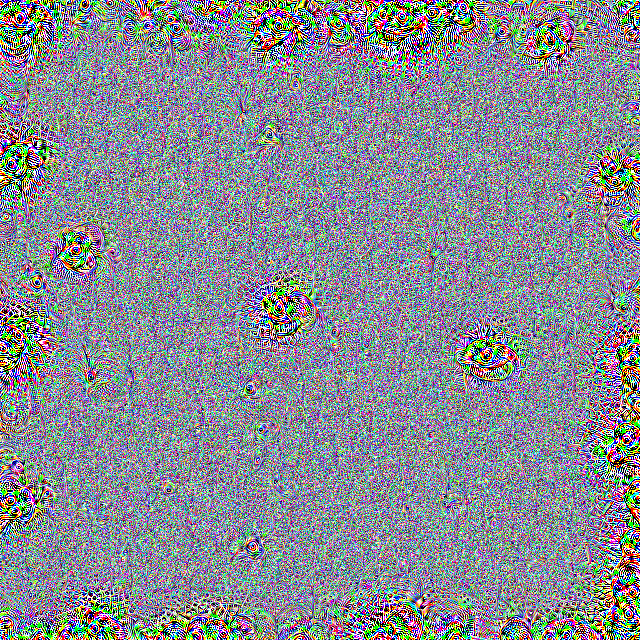
\includegraphics[width=.7\linewidth]{figuras/feat_vis/random_image_dream.png}
        \caption{Feature Visualization of Convolution layer 10 of VGG16}
    \end{subfigure}
    \hfill
    \begin{subfigure}[t]{0.28\textwidth}
        \captionsetup{justification=centering}
        \centering
        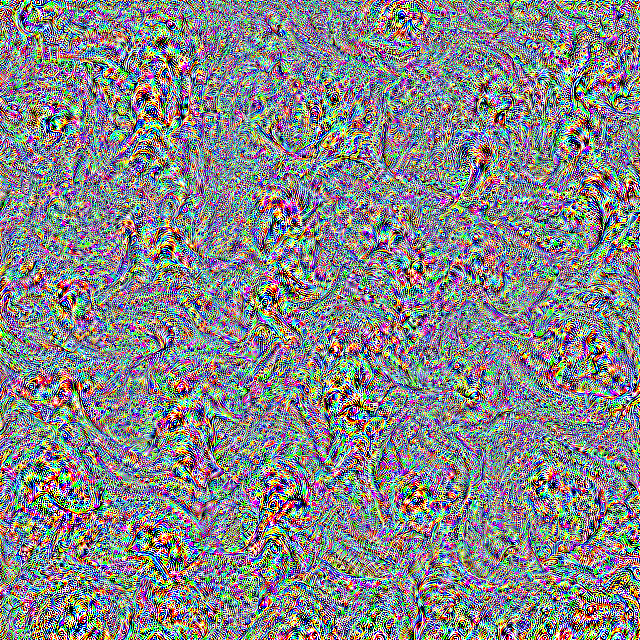
\includegraphics[width=.7\linewidth]{figuras/feat_vis/random_image_dream_class_254.png}
        \caption{Feature Visualization of Pug (ImageNet index 254) neuron of VGG16}
    \end{subfigure}

    \caption{
        Feature Visualization images using solely Gradient Ascent. 
    Little human-recognizable features are present in the resulting images
    }
\end{figure}

To identify human-aligned features in our models, we need effective techniques for generating images that closely correspond to those features. 
A closer examination reveals that Feature Visualization using solely Gradient Ascent typically produces features that occupy only small portions of the final image.

To expand these features across a larger area and create more intricate forms, we can downscale the image and apply the Gradient Ascent step. 
Once the downscaled image has been refined, it can be upscaled by a specific factor, and Gradient Ascent can be reapplied. 
\newpage
\noindent
Repeating this process until the image reaches its original size enables the generation of more detailed and compelling results, as demonstrated below:

\begin{figure}
    \captionsetup{justification=centering}

    \begin{subfigure}[t]{0.45\textwidth}
        \captionsetup{justification=centering}
        \centering
        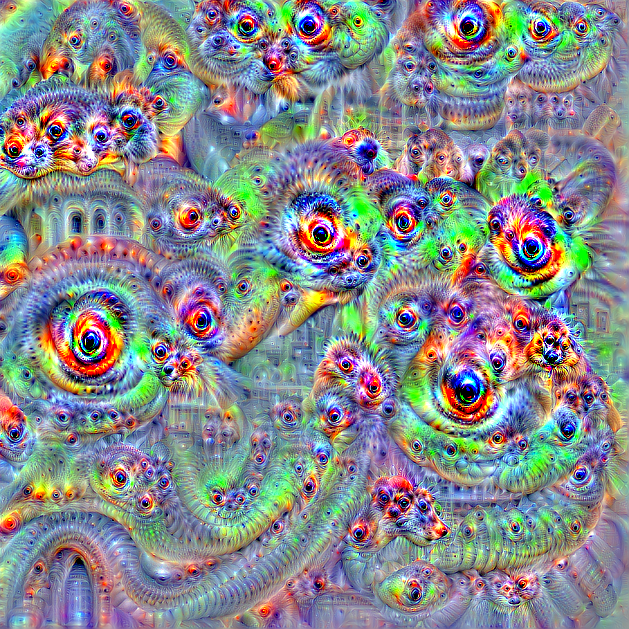
\includegraphics[width=.7\linewidth]{figuras/feat_vis/random_image_dream_pyramid.png}
        \caption{Feature Visualization of Convolution layer 10 of VGG16}
        \label{fig:feat_conv_L22_pyramid}
    \end{subfigure}
    \hfill
    \begin{subfigure}[t]{0.45\textwidth}
        \captionsetup{justification=centering}
        \centering
        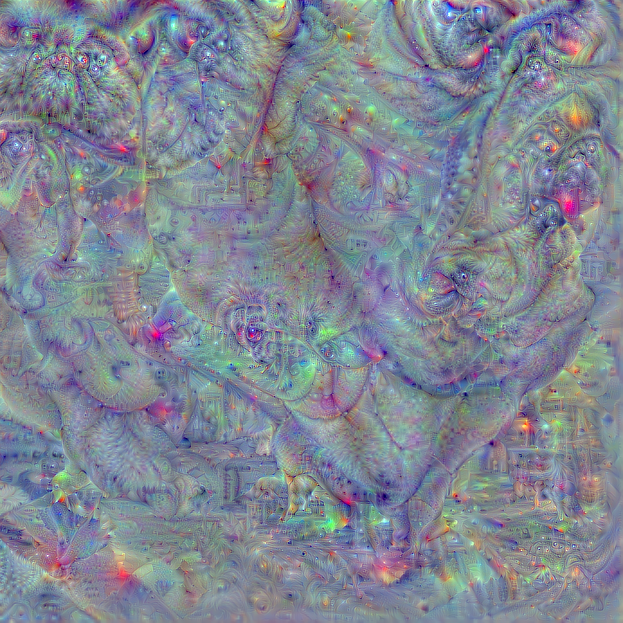
\includegraphics[width=.7\linewidth]{figuras/feat_vis/random_image_dream_pyramid_class_254.png}
        \caption{Feature Visualization of Pug (ImageNet index 254) neuron of VGG16}
        \label{fig:feat_conv_I254_pyramid}
    \end{subfigure}

    \caption{By employing Gradient Ascent across multiple image scales, we achieve results that align more closely with human perception. In Subfigure \ref{fig:feat_conv_L22_pyramid}, eye-like structures frequently emerge in the generated images, while in Subfigure \ref{fig:feat_conv_I254_pyramid}, fur-like textures (top-left portion of image) reminiscent of a Pug's facial coat are present.}
\end{figure}

Some features aligned with human perception can now be visible by applying this method on random images. 
However, high frequency noise is still very present in the generated images, a feature not very common in real life pictures.
In order to mitigate the high frequency noise, we may apply regularization techniques to the random image on every iteration of the Feature Visualization algorithm.
For example, by applying Gaussian Blur, high frequency regions are dimished because Gaussian blur is a low-pass filter.

\begin{figure}
    \captionsetup{justification=centering}

    \begin{subfigure}[t]{0.45\textwidth}
        \captionsetup{justification=centering}
        \centering
        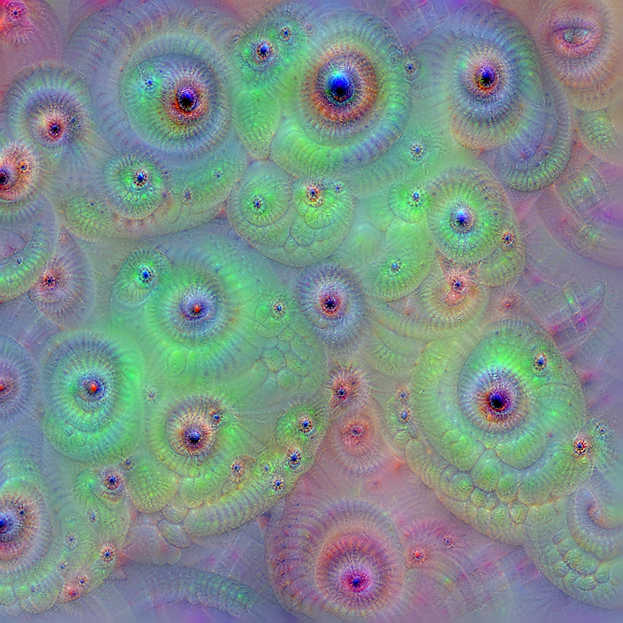
\includegraphics[width=.7\linewidth]{figuras/feat_vis/random_image_dream_reg.png}
        \caption{Feature Visualization of Convolution layer 10 of VGG16}
        \label{fig:feat_conv_L22_reg}
    \end{subfigure}
    \hfill
    \begin{subfigure}[t]{0.45\textwidth}
        \captionsetup{justification=centering}
        \centering
        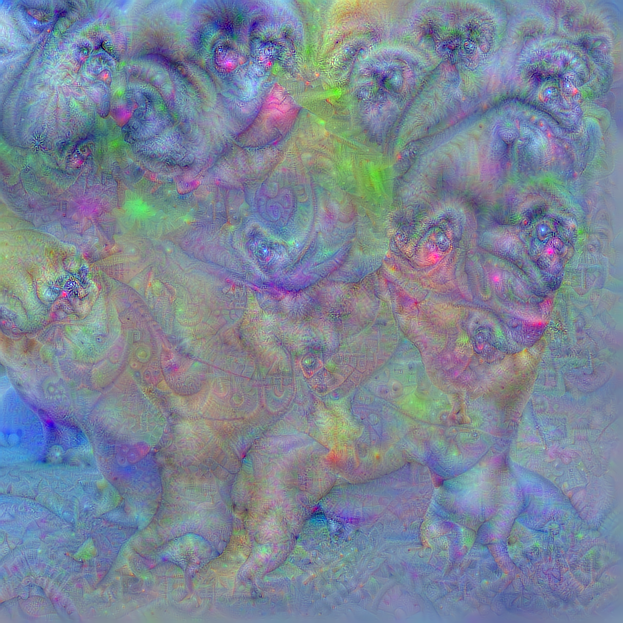
\includegraphics[width=.7\linewidth]{figuras/feat_vis/random_image_dream_pug_254_reg.png}
        \caption{Feature Visualization of Pug (ImageNet index 254) neuron of VGG16}
        \label{fig:feat_conv_I254_reg}
    \end{subfigure}

    \caption{
        Feature Visualization images generated by applying Gaussian Blur besides multi-scale Gradient Ascent. 
        This technique applied on Layer 10 predictably yields an image with much lower frequencies than \ref{fig:feat_conv_L22_pyramid}. 
        Also, patterns like snouts or eyes are still present with round and circular features. 
        As for Subfigure \ref{fig:feat_conv_I254_reg}, pug-like faces are very present in the generated image, unlike what is present in Subfigure \ref{fig:feat_conv_I254_pyramid}.   
    }
    \label{fig:feat_vis_regularization}

\end{figure}

\newpage

By incorporating regularization, as shown in Figure \ref{fig:feat_vis_regularization}, we generated more human-aligned images with clearly recognizable features.
Using the techniques found in this section, an implementation will be proposed in the next section.

\section{Implementation}

Following the theory explored in the last section, an implementation in Python using the library \href{https://pytorch.org/}{Pytorch} will be proposed in this section. 

For our experiments, we will use a VGG16 CNN architecture trained on ImageNet. The model is made available by the library \href{https://pytorch.org/vision/stable/index.html}{Torchvision}. 
We can import the model with pretrained weights with the code bellow: 

\begin{program}
    \index{Python}
    \centering

    \begin{lstlisting}[language=Python, style=wider]
        from torchvision.models import vgg16, VGG16_Weights

        model = vgg16(weights=VGG16_Weights.IMAGENET1K_V1)
    \end{lstlisting}

    \caption{Loading pretrained VGG16 model}
\end{program}

Now, we need to define a way to track activations of certain layers or neurons of the network in order optimize the Feature Visualization images. 
In Pytorch, we can define \emph{Hooks}, which will update every time a forward pass is executed in the network. 
In our implementation, we defined the following Hook class to track activations:

\begin{program}
    \index{Python}
    \centering
    \label{code:hook_class}
    \begin{lstlisting}[language=Python, style=wider]
        class Hook:
            def __init__(self, model_layer: Sequential):
                self.hook = model_layer.register_forward_hook(self.hook_fn)

            def hook_fn(self, _, input: Tensor, output: Tensor):
                self.input = input
                self.output = output
            
            def close(self):
                self.hook.remove()
    \end{lstlisting}

    \caption{Hook Class}
\end{program}

\noindent Where activations can be retrieved after each forward pass by checking the hook's output:

\begin{program}
    \index{Python}
    \centering
    \label{code:hook_usage}

    \begin{lstlisting}[language=Python, style=wider]
        model = vgg16(weights=VGG16_Weights.IMAGENET1K_V1)
        hook = Hook(model.features[22])
        model(image)        # compute forward pass in model
        activations = hook.output       # retrieve model.features[22] activations
    \end{lstlisting}

    \caption{Hook Usage}
\end{program}

\newpage
Using hooks, the Gradient Ascent step can now be implemented:

\begin{program}
    \index{Python}
    \centering
    \label{code:gradient_ascent_step}

    \begin{lstlisting}[language=Python, style=wider]
        def gradient_ascent_step(
            image: torch.Tensor,
            model: torch.nn.Module,
            hook: Hook,
            learning_rate: float
            ) -> torch.Tensor:
            
            blur = GaussianBlur(kernel_size=7, sigma=0.9)
            image = blur(image)

            image.requires_grad_()
            
            model(image)
            activations = hook.output

            loss = (activations**2).sum()

            loss.backward()
            normalized_grad = (image.grad - image.grad.mean()) / image.grad.std()

            image.grad.zero_()
            image = image.detach()
            image += learning_rate * normalized_grad

            return image
    \end{lstlisting}

    \caption{Gradient Ascent Step with Normalization}
\end{program}

\noindent The algorithm begins by applying a blur to the input image in lines 8 and 9 to regularize the results, producing a smoother and less noisy output, as discussed in the previous section.
Next, gradient computation is enabled for the image in line 11, a necessary step for handling PyTorch tensors.
Following this, the activations in the layer are calculated and aggregated into a single value in lines 13 to 16, which is then used to compute the gradient.
Finally, the gradient is computed in line 18, normalized in line 19, and the image is updated in line 23, completing one step of Gradient Ascent.

\newpage
Now, we can compute Gradient Ascent through mulitple iterations with multiple image scales, until we are satisfied with the results. 

\begin{program}
    \index{Python}
    \centering
    \label{code:feat_visualization}

    \begin{lstlisting}[language=Python, style=wider]
        def feature_visualization(
            image: torch.Tensor,
            model: torch.nn.Module,
            model_layer: torch.nn.Module,
            pyramid_levels: int,
            growth_rate: float,
            steps: int,
            learning_rate: float
        ) -> torch.Tensor: 
        
        resizer = Resizer(pyramid_levels, image)

        hook = Hook(model_layer, backward=False)
        
        for pyramid_level in range(pyramid_levels):
            image = resizer.resize(image, pyramid_level)

            for _ in range(steps):
                image = gradient_ascent_step(image, model, hook, learning_rate)
            
        image = image.clamp(0, 1)
        return image
    \end{lstlisting}

    \caption{Feature Visualization}
\end{program}

In simple terms, we create an \emph{Resizer} object responsible to rescale the image on every step of the outer for loop (line 16). 
Then, we bind the hook to the desired model layer in line 13 and process the image for each image size computed in line 16 and for the desired amount of Gradient Ascent steps for each iteration.
After the process, the image is clamped back to the interval \([0, 1]\), since the Gradient Ascent steps can bring the generated image pixels out of the interval.

\section{Experiments}

In this section, we present a series of experiments conducted to evaluate and demonstrate the effectiveness of feature visualization techniques. 
These experiments are designed to highlight the interpretability of the learned features in deep neural networks, analyze their behavior across different layers and architectures, and explore their potential applications. 
Through these experiments, we aim to provide both qualitative and quantitative insights into the representational power and limitations of feature visualization.

The experiments in this section are performed using the VGG16 convolutional neural network (CNN) architecture, pre-trained on the ImageNet dataset. 
The hyperparameters will be carefully optimized to produce results that closely align with human interpretability and understanding.

\subsection{Layer-Wise Visualization}


To create feature visualization images that capture the most significant features of an entire layer, we compute the gradient of the sum of all neuron activations within that layer. 
This approach highlights the collective importance of features across the layer.
As an initial example, feature visualization images were generated for Layer 10 of the VGG16 architecture, as shown in Figures \ref{fig:feat_conv_L22_pyramid} and \ref{fig:feat_conv_L22_reg}.
Next, we will extend this exploration to various layers of the network to analyze how features evolve throughout the architecture.

\subsubsection{Initial Layers (1-5)}


\begin{figure}
    \captionsetup{justification=centering}

    \begin{subfigure}[t]{0.31\textwidth}
        \captionsetup{justification=centering}
        \centering
        
\includegraphics[width=.7\linewidth]{figuras/feat_vis/experiments/layers/initial/l1/random_image_pl1_lr4e-1_layer0_no-blur.png}
        \caption{No Multiscaling, No Blurring, \(learning\_rate = 0.4\)}
    \end{subfigure}
    \hfill
    \begin{subfigure}[t]{0.31\textwidth}
        \captionsetup{justification=centering}
        \centering
        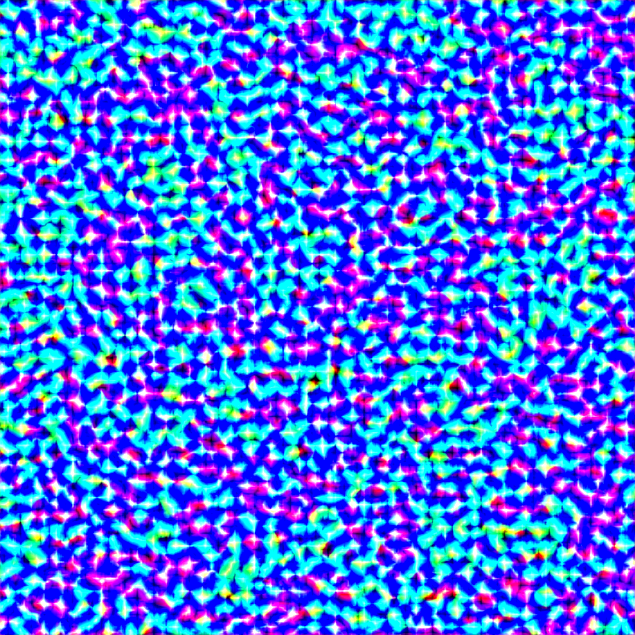
\includegraphics[width=.7\linewidth]{figuras/feat_vis/experiments/layers/initial/l1/random_image_pl4_lr4e-2_layer0_no-blur.png}
        \caption{4 Layer Multiscaling, No Blurring, \(learning\_rate = 0.04\)}
    \end{subfigure}
    \hfill
    \begin{subfigure}[t]{0.31\textwidth}
        \captionsetup{justification=centering}
        \centering
        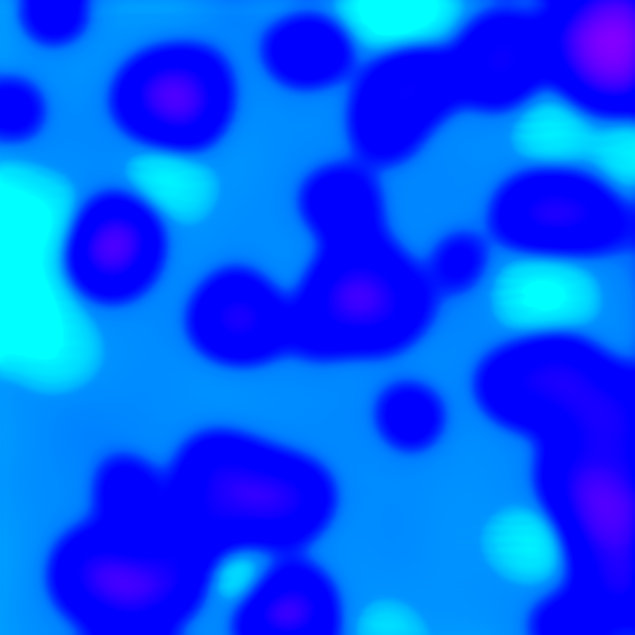
\includegraphics[width=.7\linewidth]{figuras/feat_vis/experiments/layers/initial/l1/random_image_pl4_lr4e-2_layer0.png}
        \caption{4 Layer Multiscaling, Blurring, \(learning\_rate = 0.04\)}
    \end{subfigure}

    \caption{Layer 1}
    \label{fig:layer_1}
\end{figure}

\begin{figure}
    \captionsetup{justification=centering}

    \begin{subfigure}[t]{0.31\textwidth}
        \captionsetup{justification=centering}
        \centering
        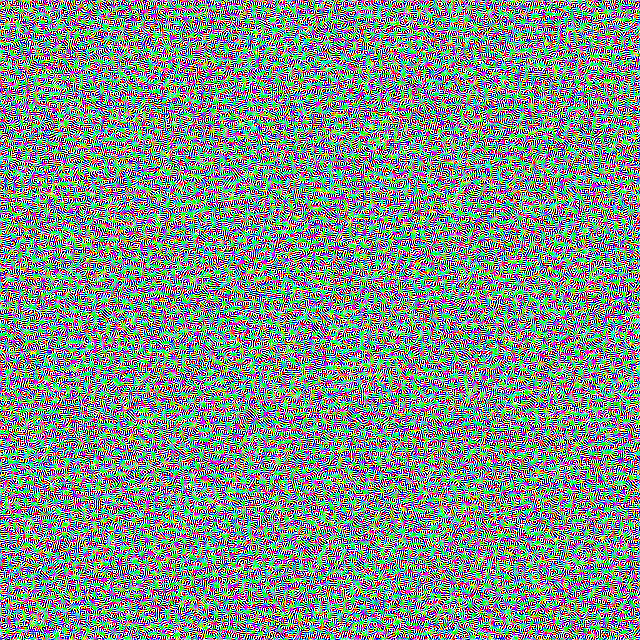
\includegraphics[width=.7\linewidth]{figuras/feat_vis/experiments/layers/initial/l3/random_image_pl1_lr4e-1_layer5_no-blur.png}
        \caption{No Multiscaling, No Blurring, \(learning\_rate = 0.4\)}
    \end{subfigure}
    \hfill
    \begin{subfigure}[t]{0.31\textwidth}
        \captionsetup{justification=centering}
        \centering
        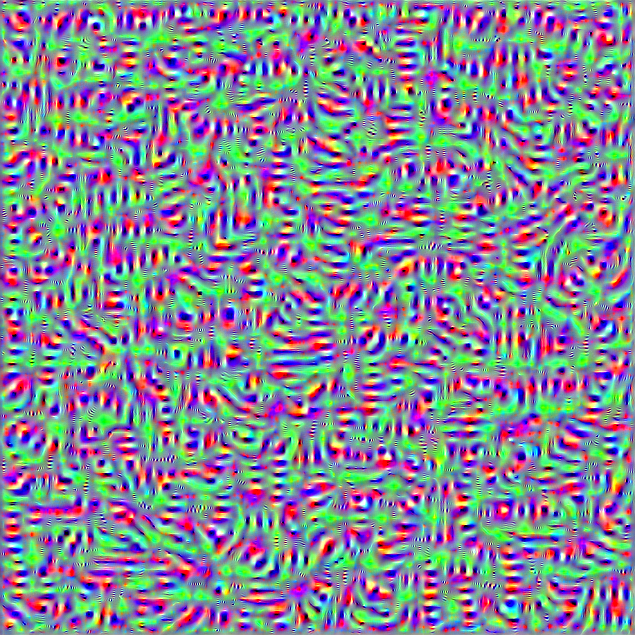
\includegraphics[width=.7\linewidth]{figuras/feat_vis/experiments/layers/initial/l3/random_image_pl4_lr4e-2_layer5_no-blur.png}
        \caption{4 Layer Multiscaling, No Blurring, \(learning\_rate = 0.04\)}
    \end{subfigure}
    \hfill
    \begin{subfigure}[t]{0.31\textwidth}
        \captionsetup{justification=centering}
        \centering
        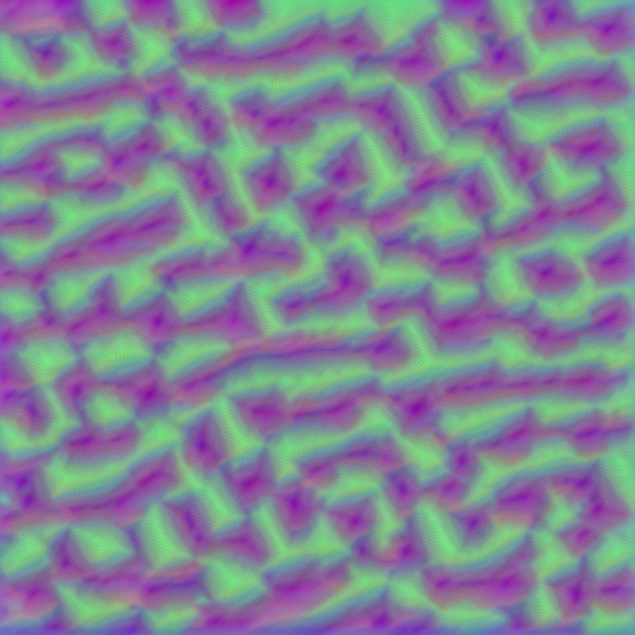
\includegraphics[width=.7\linewidth]{figuras/feat_vis/experiments/layers/initial/l3/random_image_pl4_lr4e-2_layer5.png}
        \caption{4 Layer Multiscaling, Blurring, \(learning\_rate = 0.04\)}
    \end{subfigure}

    \caption{Layer 3}
    \label{fig:layer_3}
\end{figure}

\newpage
\begin{figure}
    \captionsetup{justification=centering}

    \begin{subfigure}[t]{0.48\textwidth}
        \captionsetup{justification=centering}
        \centering
        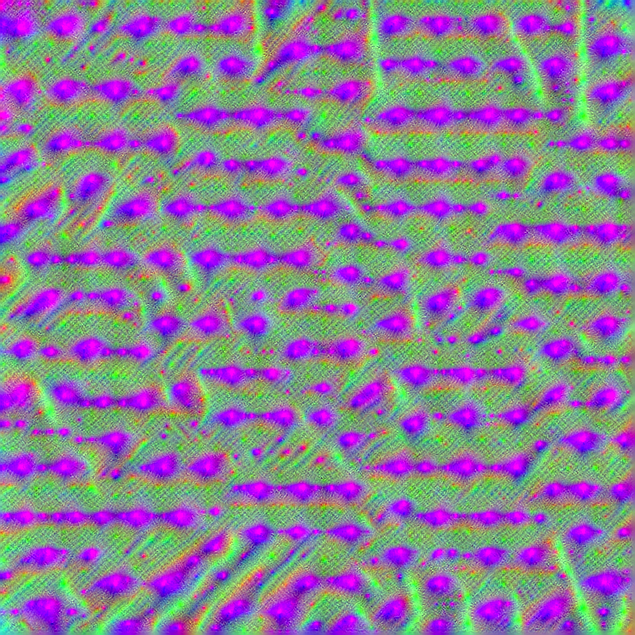
\includegraphics[width=.7\linewidth]{figuras/feat_vis/experiments/layers/initial/l5/random_image_pl4_lr2.2e-1_layer10.png}
        \caption{4 Layer Multiscaling, Blurring, \(learning\_rate = 0.22\)}
    \end{subfigure}
    \hfill
    \begin{subfigure}[t]{0.48\textwidth}
        \captionsetup{justification=centering}
        \centering
        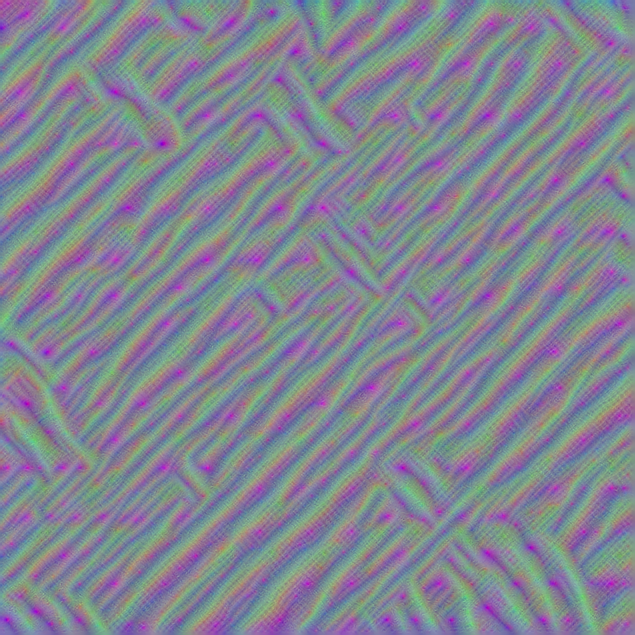
\includegraphics[width=.7\linewidth]{figuras/feat_vis/experiments/layers/initial/l5/random_image_pl4_lr8e-2_layer10.png}
        \caption{4 Layer Multiscaling, Blurring, \(learning\_rate = 0.08\)}
    \end{subfigure}

    \caption{Layer 5}
    \label{fig:layer_5}
\end{figure}

Intuitively, the initial layers of a CNN capture more simple features from images, like edges and simple formats.
By analyzing the generated images, one can clearly notice the complexity enhancement throughout the layers of the network. 
For layer 1 (Figure \ref{fig:layer_1}), the generated images mainly focus on maximizing a color value similar to blue, probably correlated to the color distribution of the images on ImageNet.
However, in layers 3 (Figure \ref{fig:layer_3}) and 5 (Figure \ref{fig:layer_5}) some patterns are already noticeable in the figures, with patterns similar to lines and curves being created.

\subsubsection{Intermediary Layers (6-9)}


\begin{figure}
    \captionsetup{justification=centering}
    
    \begin{subfigure}[t]{0.31\textwidth}
        \captionsetup{justification=centering}
        \centering
        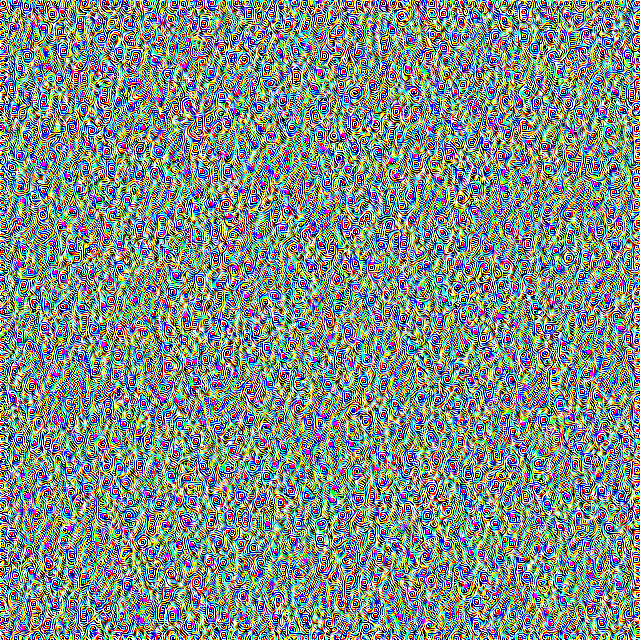
\includegraphics[width=.7\linewidth]{figuras/feat_vis/experiments/layers/intermediary/l6/random_image_pl1_lr4e-1_layer12_no-blur.png}
        \caption{No Multiscaling, No Blurring, \(learning\_rate = 0.4\)}
    \end{subfigure}
    \hfill
    \begin{subfigure}[t]{0.31\textwidth}
        \captionsetup{justification=centering}
        \centering
        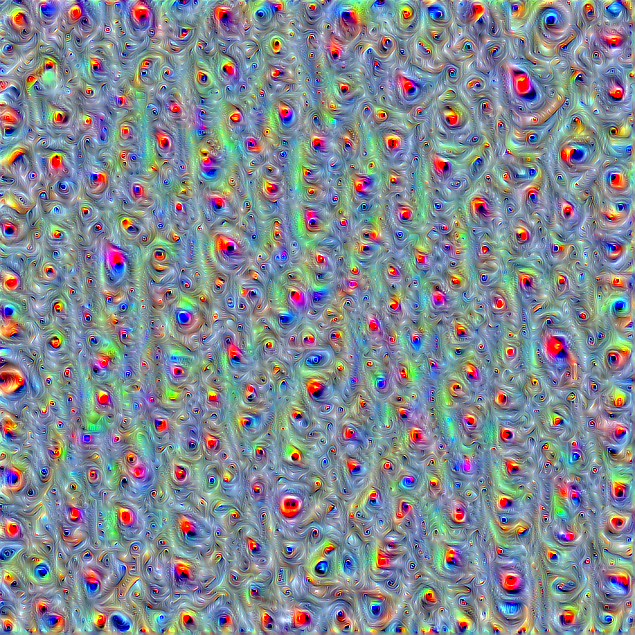
\includegraphics[width=.7\linewidth]{figuras/feat_vis/experiments/layers/intermediary/l6/random_image_pl4_lr4e-2_layer12_no-blur.png}
        \caption{4 Layer Multiscaling, No Blurring, \(learning\_rate = 0.04\)}
    \end{subfigure}
    \hfill
    \begin{subfigure}[t]{0.31\textwidth}
        \captionsetup{justification=centering}
        \centering
        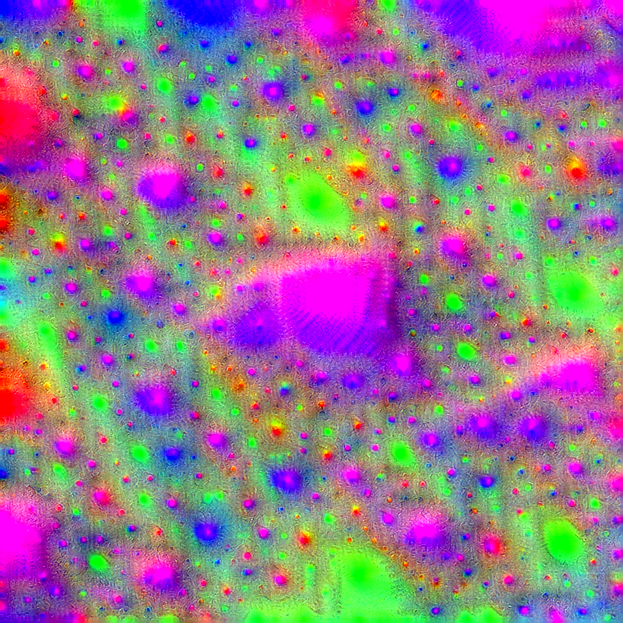
\includegraphics[width=.7\linewidth]{figuras/feat_vis/experiments/layers/intermediary/l6/random_image_pl6_lr2.2e-1_layer12.png}
        \caption{6 Layer Multiscaling, Blurring, \(learning\_rate = 0.22\)}
    \end{subfigure}
    
    \caption{Layer 6}
    \label{fig:layer_6}
\end{figure}
\begin{figure}
    \captionsetup{justification=centering}

    \begin{subfigure}[t]{0.31\textwidth}
        \captionsetup{justification=centering}
        \centering
        
\includegraphics[width=.7\linewidth]{figuras/feat_vis/experiments/layers/intermediary/l8/random_image_pl1_lr4e-1_layer17_no-blur.png}
        \caption{No Multiscaling, No Blurring, \(learning\_rate = 0.4\)}
    \end{subfigure}
    \hfill
    \begin{subfigure}[t]{0.31\textwidth}
        \captionsetup{justification=centering}
        \centering
        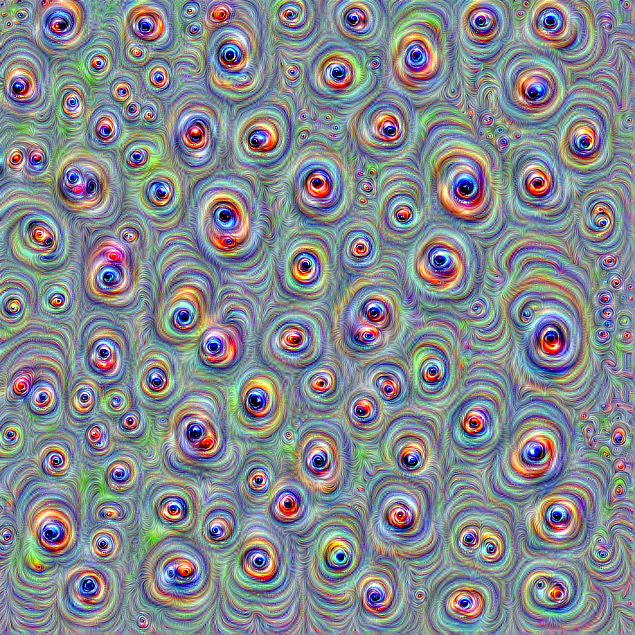
\includegraphics[width=.7\linewidth]{figuras/feat_vis/experiments/layers/intermediary/l8/random_image_pl4_lr4e-2_layer17_no-blur.png}
        \caption{4 Layer Multiscaling, No Blurring, \(learning\_rate = 0.04\)}
    \end{subfigure}
    \hfill
    \begin{subfigure}[t]{0.31\textwidth}
        \captionsetup{justification=centering}
        \centering
        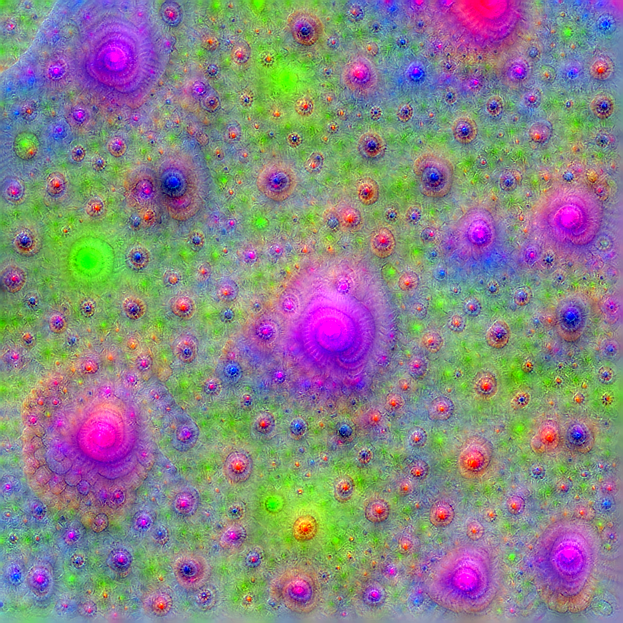
\includegraphics[width=.7\linewidth]{figuras/feat_vis/experiments/layers/intermediary/l8/random_image_pl6_lr2.2e-1_layer17.png}
        \caption{6 Layer Multiscaling, Blurring, \(learning\_rate = 0.22\)}
    \end{subfigure}

    \caption{Layer 8}
    \label{fig:layer_8}
\end{figure}


\newpage
\begin{figure}
    \captionsetup{justification=centering}
    
    \begin{subfigure}[t]{0.31\textwidth}
        \captionsetup{justification=centering}
        \centering
        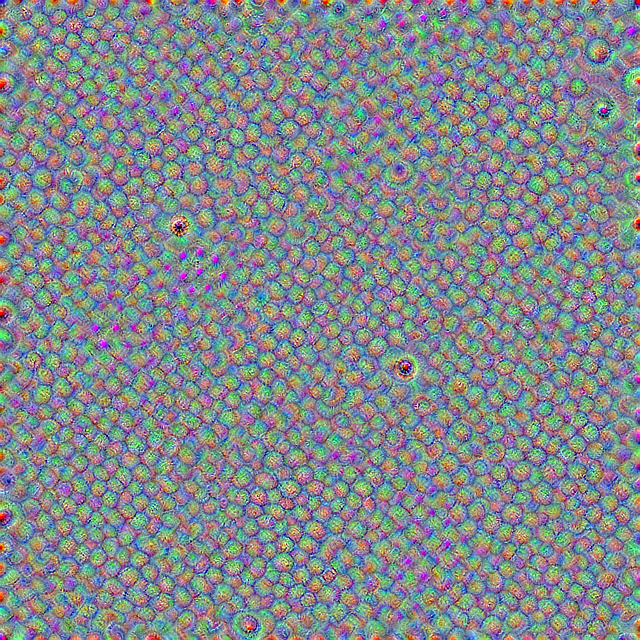
\includegraphics[width=.7\linewidth]{figuras/feat_vis/experiments/layers/intermediary/l9/random_image_pl1_lr4e-1_layer19.png}
        \caption{No Multiscaling, Blurring, \(learning\_rate = 0.4\)}
    \end{subfigure}
    \hfill
    \begin{subfigure}[t]{0.31\textwidth}
        \captionsetup{justification=centering}
        \centering
        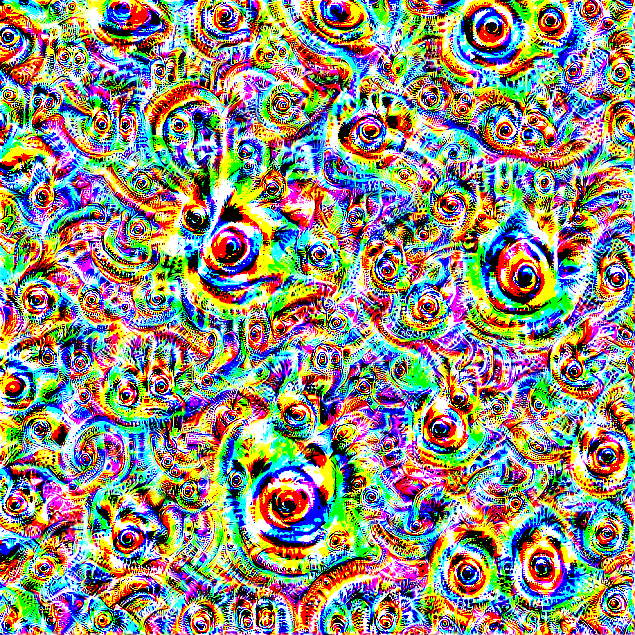
\includegraphics[width=.7\linewidth]{figuras/feat_vis/experiments/layers/intermediary/l9/random_image_pl4_lr4e-1_layer19_no-blur.png}
        \caption{4 Layer Multiscaling, No Blurring, \(learning\_rate = 0.4\)}
    \end{subfigure}
    \hfill
    \begin{subfigure}[t]{0.31\textwidth}
        \captionsetup{justification=centering}
        \centering
        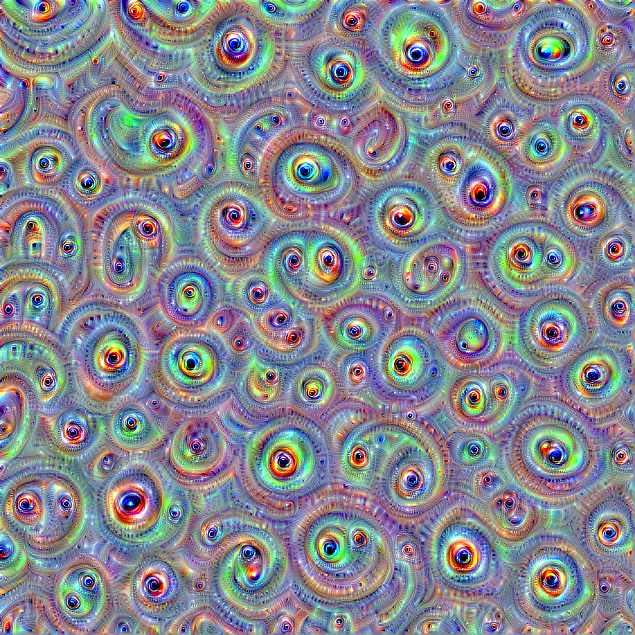
\includegraphics[width=.7\linewidth]{figuras/feat_vis/experiments/layers/intermediary/l9/random_image_pl4_lr4e-2_layer19_no-blur.png}
        \caption{4 Layer Multiscaling, No Blurring, \(learning\_rate = 0.04\)}
    \end{subfigure}
    
    \caption{Layer 9}
    \label{fig:layer_9}
    
\end{figure}

From our experiments, we can observe that complex features emerge from intermediary layers, with eye-like patterns appearing in Figures \ref{fig:layer_8} and \ref{fig:layer_9}, probably related to the huge amount of animal pictures in the training dataset.
Also, curves and circles are way more present in this layer range, showing that the network learned throughout its layers to maximize its activation to more \emph{curvy patterns}, since real life pictures tend to have less linear line segments. 

\subsubsection{Final Layers (10-13)}

\begin{figure}
    \captionsetup{justification=centering}
    
    \begin{subfigure}[t]{0.42\textwidth}
        \captionsetup{justification=centering}
        \centering
        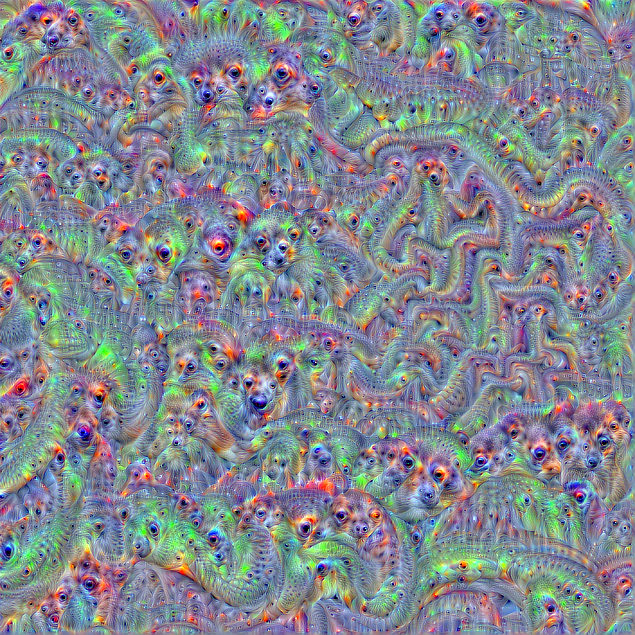
\includegraphics[width=.7\linewidth]{figuras/feat_vis/experiments/layers/final/l10/random_image_pl4_lr4e-2_layer21_no-blur.png}
        \caption{4 Layer Multiscaling, No Blurring, \(learning\_rate = 0.04\)}
    \end{subfigure}
    \hfill
    \begin{subfigure}[t]{0.42\textwidth}
        \captionsetup{justification=centering}
        \centering
        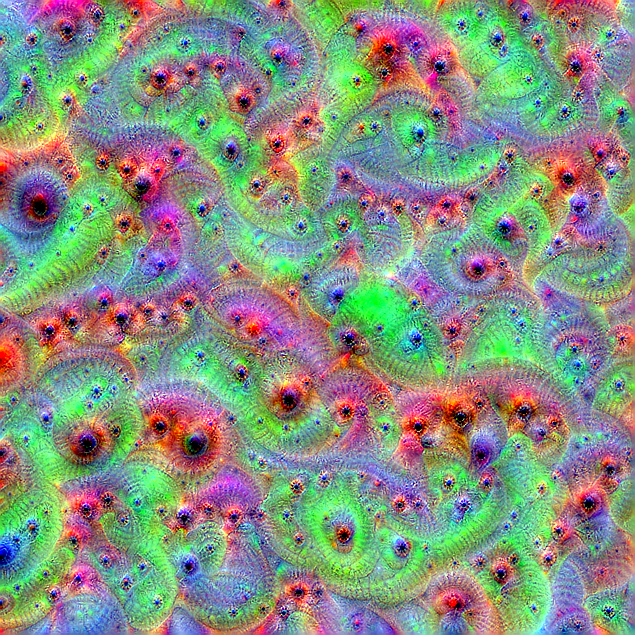
\includegraphics[width=.7\linewidth]{figuras/feat_vis/experiments/layers/final/l10/random_image_pl4_lr4e-1_layer21.png}
        \caption{4 Layer Multiscaling, Blurring, \(learning\_rate = 0.4\)}
    \end{subfigure}
    
    \caption{Layer 10}
    \label{fig:layer_10}
\end{figure}

\begin{figure}
    \captionsetup{justification=centering}

    \begin{subfigure}[t]{0.31\textwidth}
        \captionsetup{justification=centering}
        \centering
        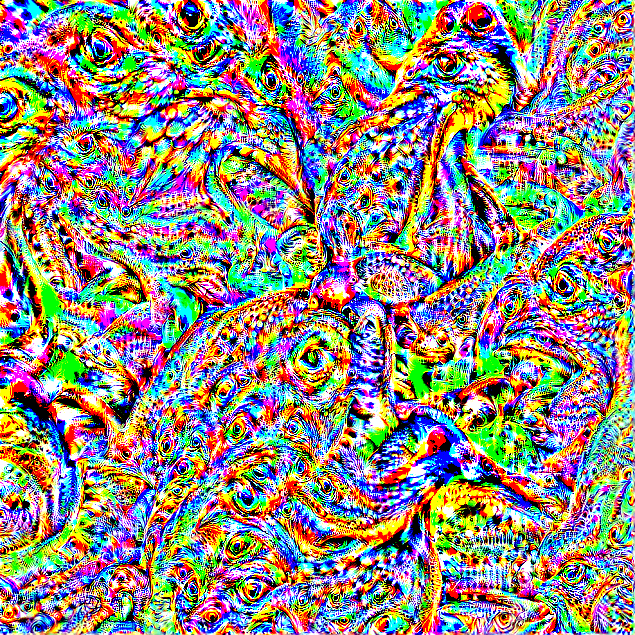
\includegraphics[width=.7\linewidth]{figuras/feat_vis/experiments/layers/final/l12/random_image_pl4_lr4e-1_layer26_no-blur.png}
        \caption{4 Layer Multiscaling, No Blurring, \(learning\_rate = 0.4\)}
    \end{subfigure}
    \hfill
    \begin{subfigure}[t]{0.31\textwidth}
        \captionsetup{justification=centering}
        \centering
        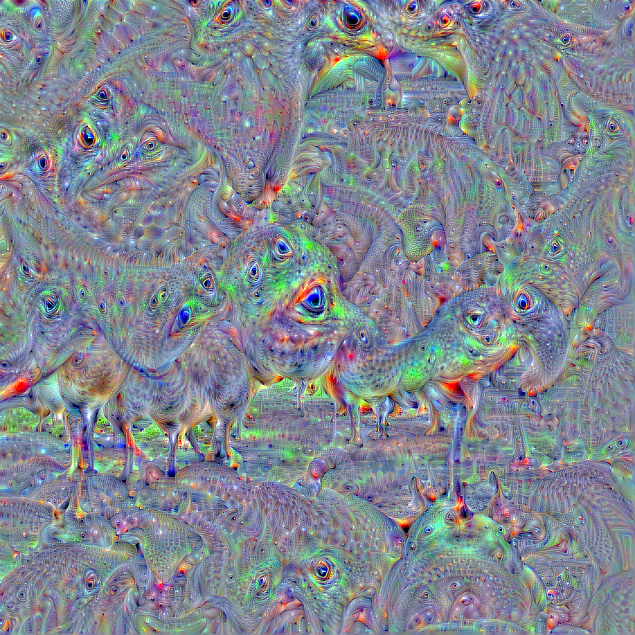
\includegraphics[width=.7\linewidth]{figuras/feat_vis/experiments/layers/final/l12/random_image_pl4_lr4e-2_layer26_no-blur.png}
        \caption{4 Layer Multiscaling, No Blurring, \(learning\_rate = 0.04\)}
    \end{subfigure}
    \hfill
    \begin{subfigure}[t]{0.31\textwidth}
        \captionsetup{justification=centering}
        \centering
        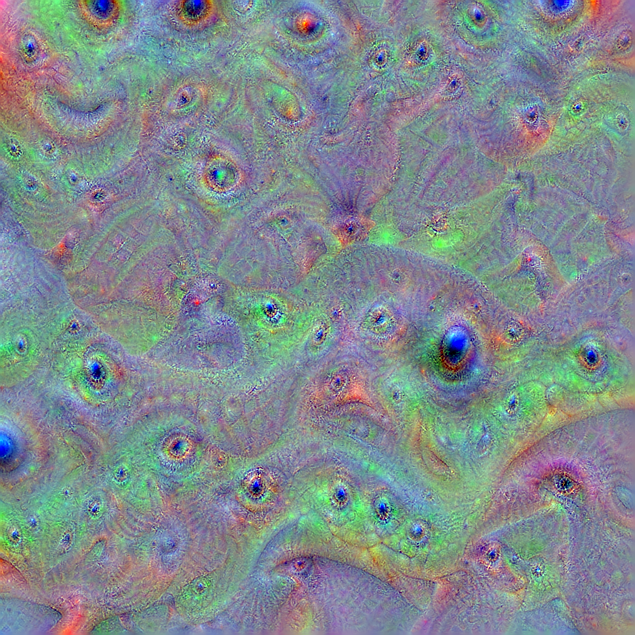
\includegraphics[width=.7\linewidth]{figuras/feat_vis/experiments/layers/final/l12/random_image_pl4_lr2.2e-1_layer26.png}
        \caption{4 Layer Multiscaling, Blurring, \(learning\_rate = 0.22\)}
    \end{subfigure}
    \hfill
    \begin{subfigure}[t]{0.31\textwidth}
        \captionsetup{justification=centering}
        \centering
        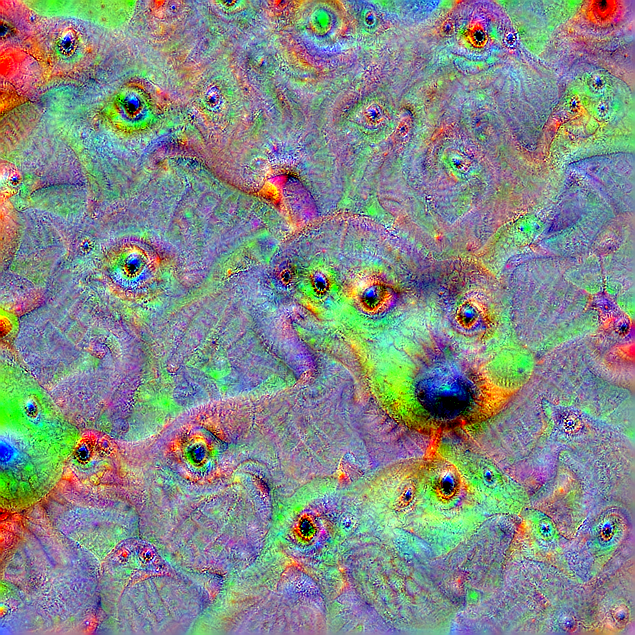
\includegraphics[width=.7\linewidth]{figuras/feat_vis/experiments/layers/final/l12/random_image_pl4_lr4e-1_layer26.png}
        \caption{4 Layer Multiscaling, Blurring, \(learning\_rate = 0.4\)}
    \end{subfigure}
    \begin{subfigure}[t]{0.31\textwidth}
        \captionsetup{justification=centering}
        \centering
        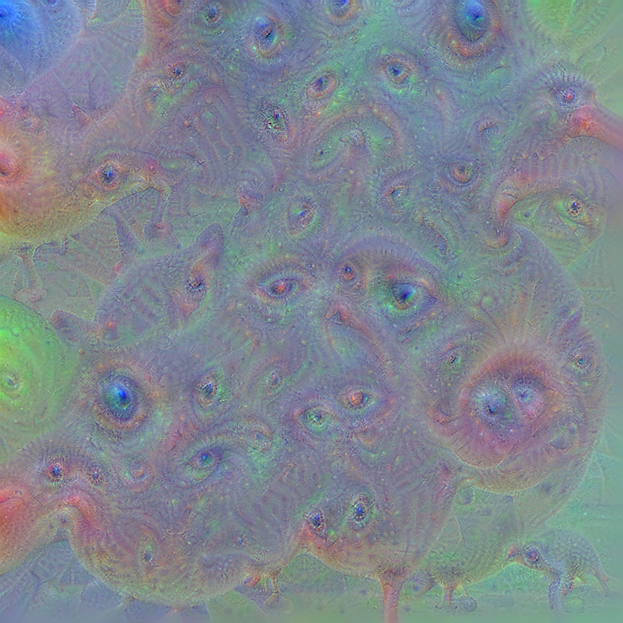
\includegraphics[width=.7\linewidth]{figuras/feat_vis/experiments/layers/final/l12/random_image_pl6_lr1e-1_layer26.png}
        \caption{6 Layer Multiscaling, Blurring, \(learning\_rate = 0.1\)}
    \end{subfigure}

    \caption{Layer 12}
    \label{fig:layer_12}
\end{figure}

\newpage
\begin{figure}
    \captionsetup{justification=centering}

    \begin{subfigure}[t]{0.31\textwidth}
        \captionsetup{justification=centering}
        \centering
        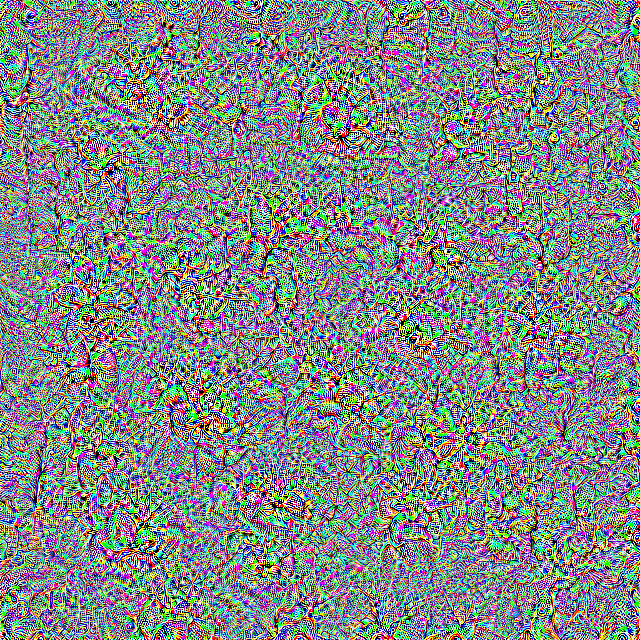
\includegraphics[width=.7\linewidth]{figuras/feat_vis/experiments/layers/final/l13/random_image_pl1_lr4e-1_layer28_no-blur.png}
        \caption{No Multiscaling, No Blurring, \(learning\_rate = 0.4\)}
    \end{subfigure}
    \hfill
    \begin{subfigure}[t]{0.31\textwidth}
        \captionsetup{justification=centering}
        \centering
        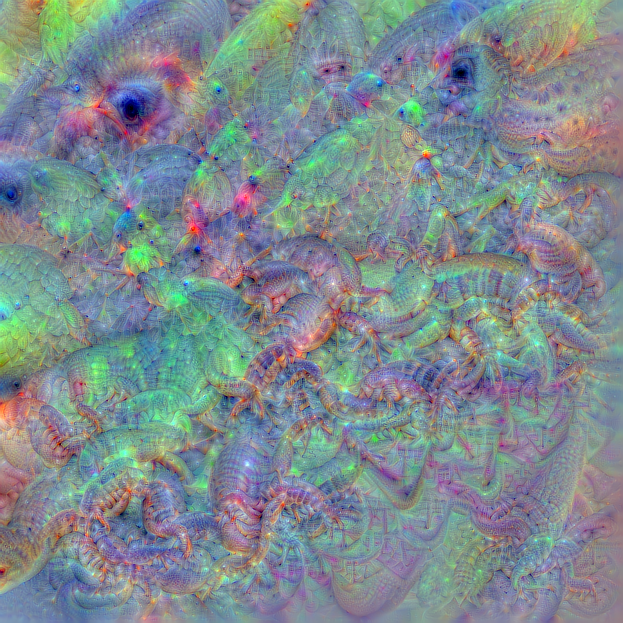
\includegraphics[width=.7\linewidth]{figuras/feat_vis/experiments/layers/final/l13/random_image_pl6_lr8e-2_layer28_blur-0.4.png}
        \caption{6 Layer Multiscaling, Blurring, \(learning\_rate = 0.08\)}
    \end{subfigure}
    \hfill
    \begin{subfigure}[t]{0.31\textwidth}
        \captionsetup{justification=centering}
        \centering
        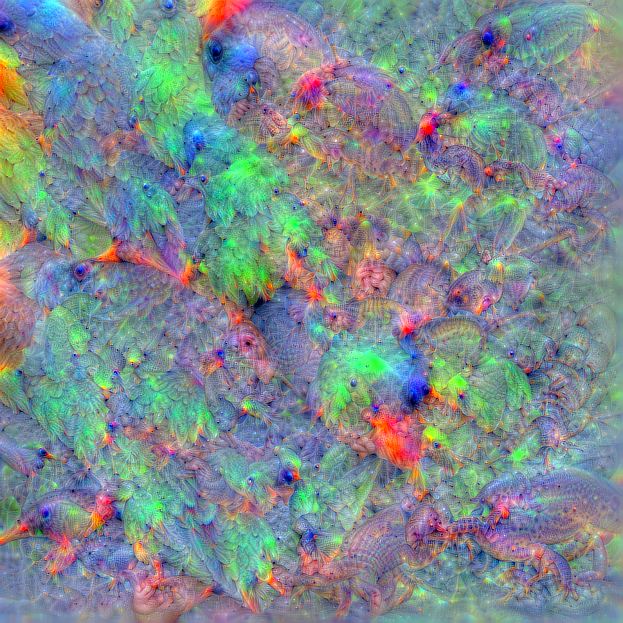
\includegraphics[width=.7\linewidth]{figuras/feat_vis/experiments/layers/final/l13/random_image_pl6_lr1e-1_layer28_blur-0.4.png}
        \caption{6 Layer Multiscaling, Blurring, \(learning\_rate = 0.1\)}
    \end{subfigure}

    \caption{Layer 13}
    \label{fig:layer_13}
\end{figure}
 
On the final layers of the network, it is possible to see that not only complex shapes are being generated but complete forms that appear like animals are also present.
For example, in Figure \ref{fig:layer_12}, in image (d), a pattern very close to a dog's muzzle is present close to the center of the image. 
Also, for image (c) in the same layer, patterns like birds faces are also recognizable in the picture.

\subsection{Class Visualization}

By maximizing the activation of a neuron corresponding to a specific class, we can generate images that visually represent the model's understanding of each class. 
This approach helps assess whether the model accurately captures the defining characteristics of each class, rather than relying on unrelated noisy biases potentially present in the dataset.

An initial example of this technique is illustrated in Figures \ref{fig:feat_conv_I254_pyramid} and \ref{fig:feat_conv_I254_reg}. 
Next, we will examine various classes using different hyperparameter configurations to explore the method further.

\subsubsection{Class 1 - Goldfish}

\begin{figure}
    \captionsetup{justification=centering}

    \begin{subfigure}[t]{0.31\textwidth}
        \captionsetup{justification=centering}
        \centering
        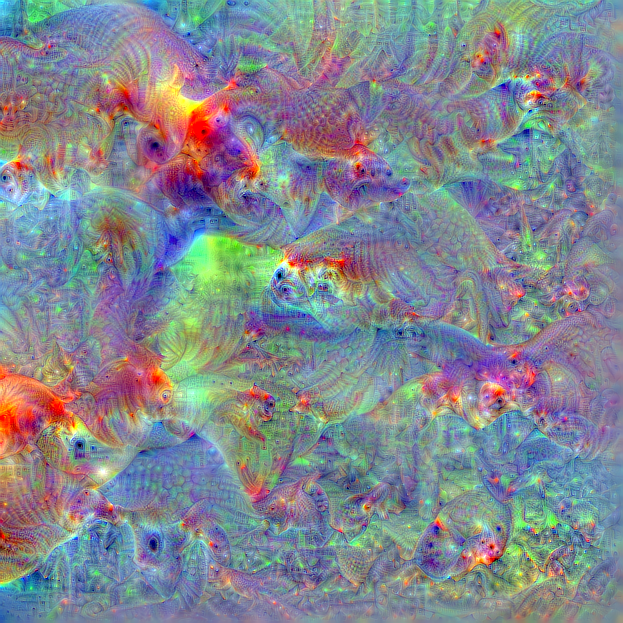
\includegraphics[width=.7\linewidth]{figuras/feat_vis/experiments/classes/cl1/random_image_ci1_lr1e-1_pl6.png}
        \caption{6 Layer Multiscaling, Blurring, \(learning\_rate = 0.1\)}
    \end{subfigure}
    \hfill
    \begin{subfigure}[t]{0.31\textwidth}
        \captionsetup{justification=centering}
        \centering
        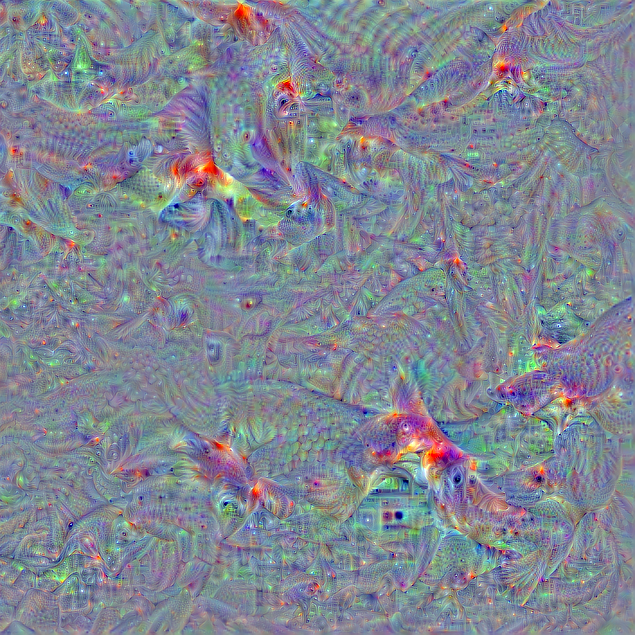
\includegraphics[width=.7\linewidth]{figuras/feat_vis/experiments/classes/cl1/random_image_ci1_lr4e-2_pl4_no-blur.png}
        \caption{4 Layer Multiscaling, No Blurring, \(learning\_rate = 0.04\)}
    \end{subfigure}
    \hfill
    \begin{subfigure}[t]{0.31\textwidth}
        \captionsetup{justification=centering}
        \centering
        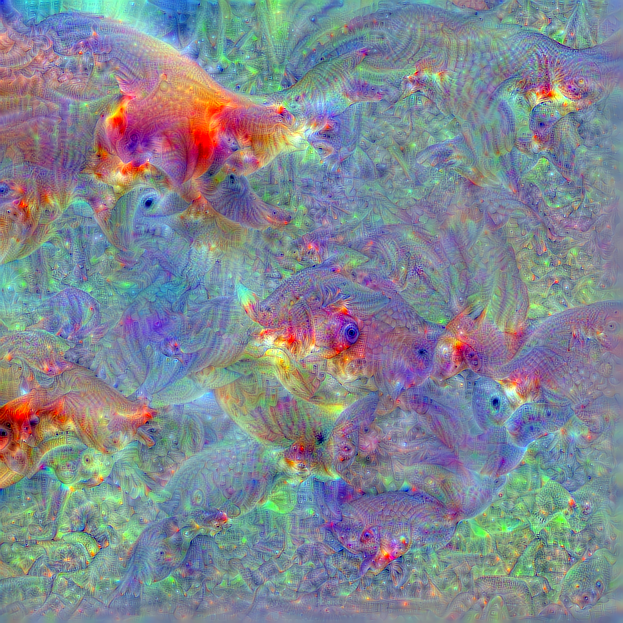
\includegraphics[width=.7\linewidth]{figuras/feat_vis/experiments/classes/cl1/random_image_ci1_lr9e-2_pl6.png}
        \caption{6 Layer Multiscaling, Blurring, \(learning\_rate = 0.09\)}
    \end{subfigure}

    \caption{Goldfish Class Feature Visualization for VGG16}
    \label{fig:class_goldfish}
\end{figure}

It is possible to notice in the generated images the characteristic orange color of Goldfishes, followed by eye-like shapes and patterns similar to a fish's scales.

\subsubsection{Class 33 - Turtle}

\begin{figure}
    \captionsetup{justification=centering}

    \begin{subfigure}[t]{0.46\textwidth}
        \captionsetup{justification=centering}
        \centering
        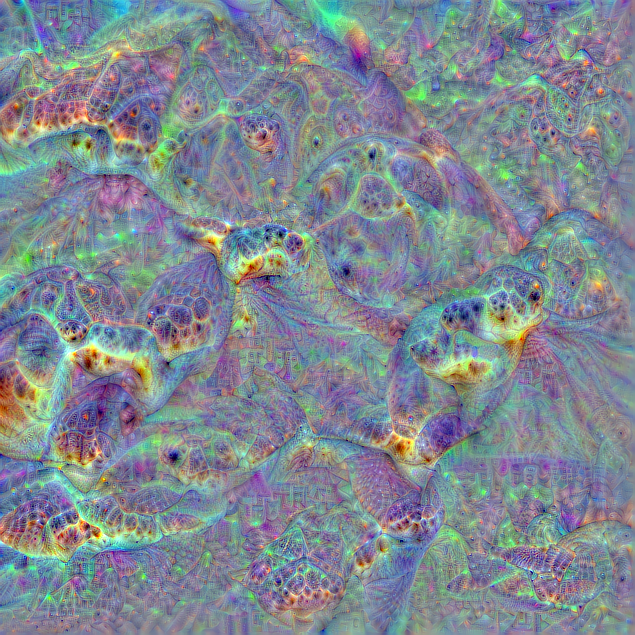
\includegraphics[width=.7\linewidth]{figuras/feat_vis/experiments/classes/cl33/random_image_ci33_lr1e-1_pl4.png}
        \caption{4 Layer Multiscaling, Blurring, \(learning\_rate = 0.1\)}
    \end{subfigure}
    \hfill
    \begin{subfigure}[t]{0.46\textwidth}
        \captionsetup{justification=centering}
        \centering
        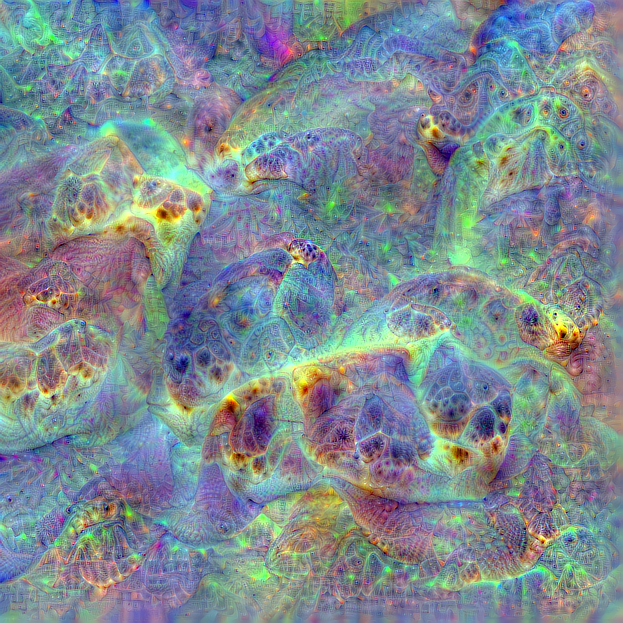
\includegraphics[width=.7\linewidth]{figuras/feat_vis/experiments/classes/cl33/random_image_ci33_lr1e-1_pl6.png}
        \caption{6 Layer Multiscaling, Blurring, \(learning\_rate = 0.1\)}
    \end{subfigure}

    \caption{Turtle Class Feature Visualization for VGG16}
    \label{fig:class_turtle}
\end{figure}


The generated images feature the distinctive skin patterns of a turtle, but no recognizable turtle face is visible.

\newpage
\subsubsection{Class 77 - Spider}

\begin{figure}
    \captionsetup{justification=centering}

    \begin{subfigure}[t]{0.46\textwidth}
        \captionsetup{justification=centering}
        \centering
        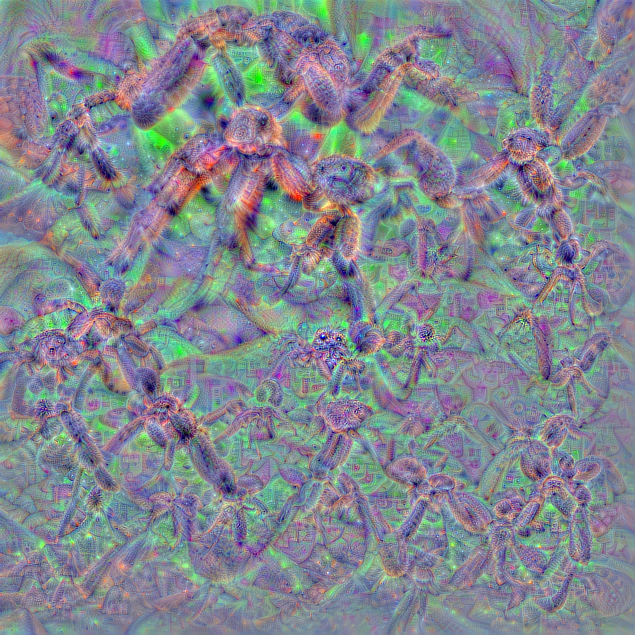
\includegraphics[width=.7\linewidth]{figuras/feat_vis/experiments/classes/cl77/random_image_ci77_lr1e-1_pl4.png}
        \caption{4 Layer Multiscaling, Blurring, \(learning\_rate = 0.1\)}
    \end{subfigure}
    \hfill
    \begin{subfigure}[t]{0.46\textwidth}
        \captionsetup{justification=centering}
        \centering
        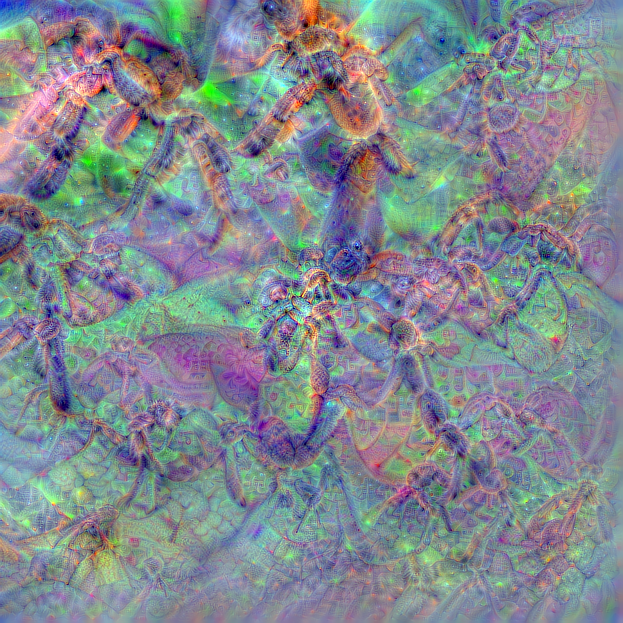
\includegraphics[width=.7\linewidth]{figuras/feat_vis/experiments/classes/cl77/random_image_ci77_lr1e-1_pl6.png}
        \caption{6 Layer Multiscaling, Blurring, \(learning\_rate = 0.1\)}
    \end{subfigure}
    \hfill
    \begin{subfigure}[t]{0.46\textwidth}
        \captionsetup{justification=centering}
        \centering
        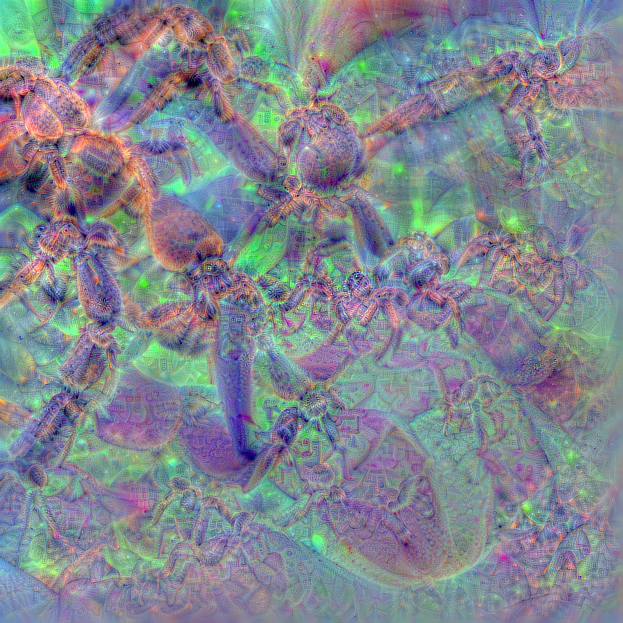
\includegraphics[width=.7\linewidth]{figuras/feat_vis/experiments/classes/cl77/random_image_ci77_lr9e-2_pl6.png}
        \caption{6 Layer Multiscaling, Blurring, \(learning\_rate = 0.09\)}
    \end{subfigure}
    \hfill
    \begin{subfigure}[t]{0.46\textwidth}
        \captionsetup{justification=centering}
        \centering
        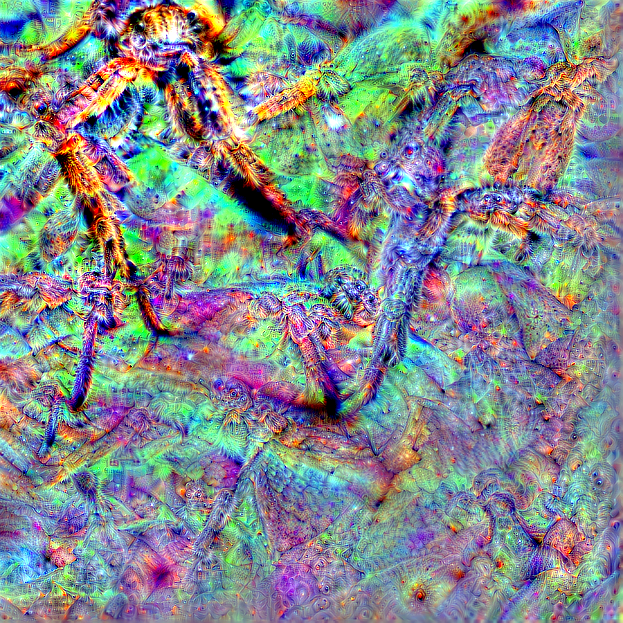
\includegraphics[width=.7\linewidth]{figuras/feat_vis/experiments/classes/cl77/random_image_ci77_lr9e-2_pl6_no-blur.png}
        \caption{6 Layer Multiscaling, No Blurring, \(learning\_rate = 0.09\)}
    \end{subfigure}

    \caption{Spider Class Feature Visualization for VGG16}
    \label{fig:class_spider}
\end{figure}

A spider's complete anatomy is visible throughout the generated images, with the arachnid's hairy limbs clearly visible at different angles.  

\newpage
\subsubsection{Class 207 - Golder Retriever}

\begin{figure}
    \captionsetup{justification=centering}

    \begin{subfigure}[t]{0.31\textwidth}
        \captionsetup{justification=centering}
        \centering
        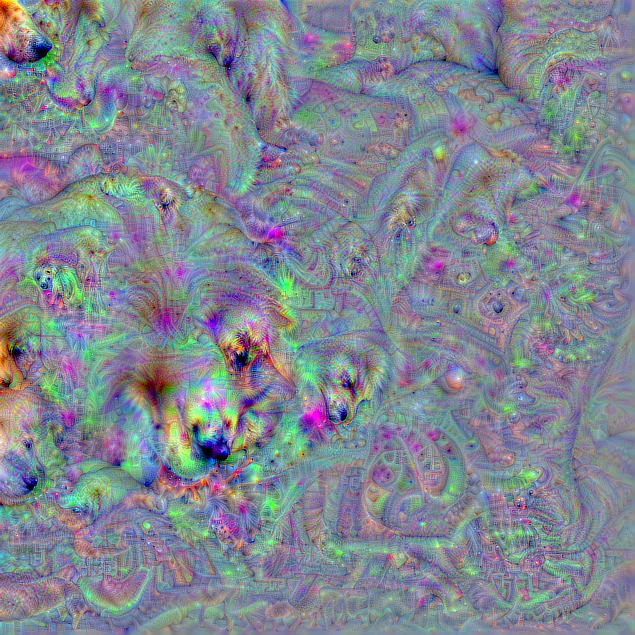
\includegraphics[width=.7\linewidth]{figuras/feat_vis/experiments/classes/cl207/random_image_ci207_lr1e-1_pl4.png}
        \caption{4 Layer Multiscaling, Blurring, \(learning\_rate = 0.1\)}
    \end{subfigure}
    \hfill
    \begin{subfigure}[t]{0.31\textwidth}
        \captionsetup{justification=centering}
        \centering
        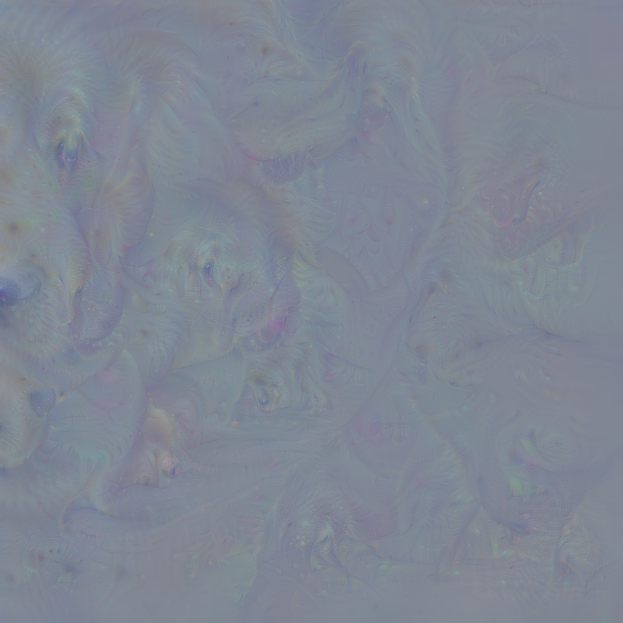
\includegraphics[width=.7\linewidth]{figuras/feat_vis/experiments/classes/cl207/random_image_ci207_lr1e-2_pl6.png}
        \caption{6 Layer Multiscaling, Blurring, \(learning\_rate = 0.01\)}
    \end{subfigure}
    \hfill
    \begin{subfigure}[t]{0.31\textwidth}
        \captionsetup{justification=centering}
        \centering
        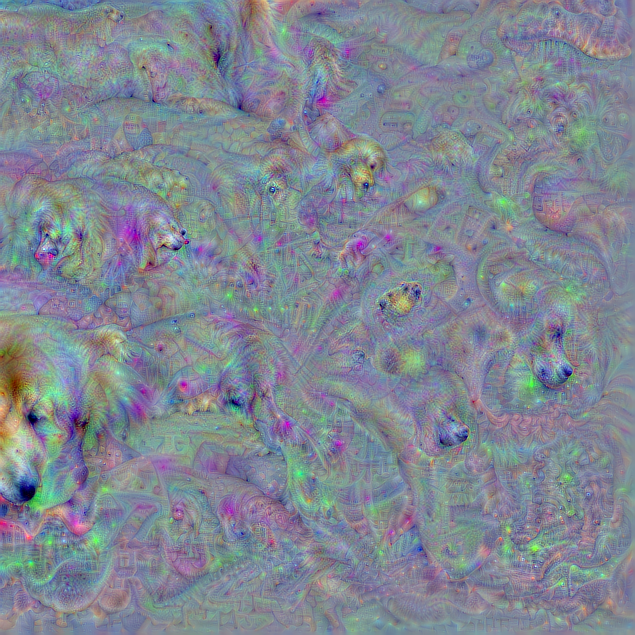
\includegraphics[width=.7\linewidth]{figuras/feat_vis/experiments/classes/cl207/random_image_ci207_lr7e-2_pl4.png}
        \caption{4 Layer Multiscaling, Blurring, \(learning\_rate = 0.07\)}
    \end{subfigure}

    \caption{Golden Retriever Class Feature Visualization for VGG16}
    \label{fig:class_golden_retriever}
\end{figure}

The generated images predominantly feature fur patterns and facial details of a golden retriever, with image (b) displaying a structure resembling a complete golden retriever face on the left.

\subsubsection{Class 254 - Pug}

\begin{figure}
    \captionsetup{justification=centering}

    \begin{subfigure}[t]{0.31\textwidth}
        \captionsetup{justification=centering}
        \centering
        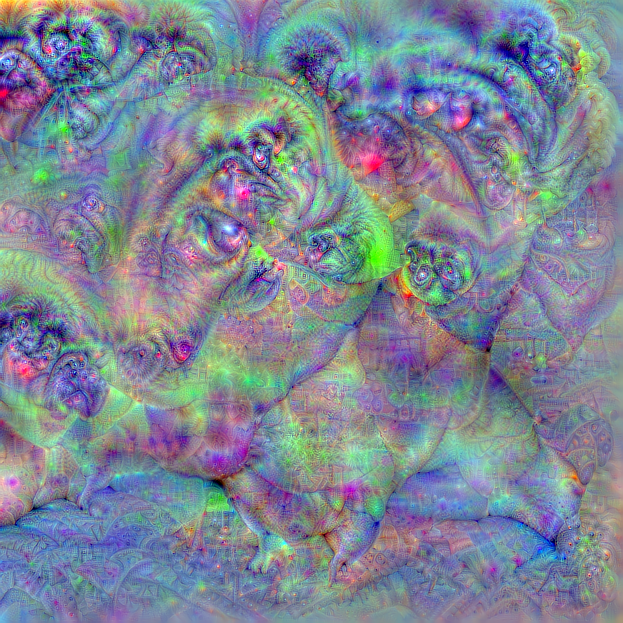
\includegraphics[width=.7\linewidth]{figuras/feat_vis/experiments/classes/cl254/random_image_ci254_lr1e-1_pl6.png}
        \caption{6 Layer Multiscaling, Blurring, \(learning\_rate = 0.1\)}
    \end{subfigure}
    \hfill
    \begin{subfigure}[t]{0.31\textwidth}
        \captionsetup{justification=centering}
        \centering
        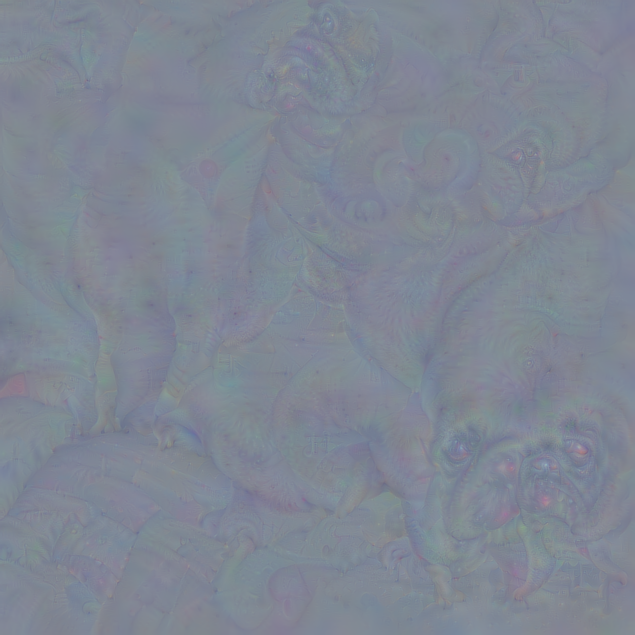
\includegraphics[width=.7\linewidth]{figuras/feat_vis/experiments/classes/cl254/random_image_ci254_lr1e-2_pl4.png}
        \caption{4 Layer Multiscaling, Blurring, \(learning\_rate = 0.01\)}
    \end{subfigure}
    \hfill
    \begin{subfigure}[t]{0.31\textwidth}
        \captionsetup{justification=centering}
        \centering
        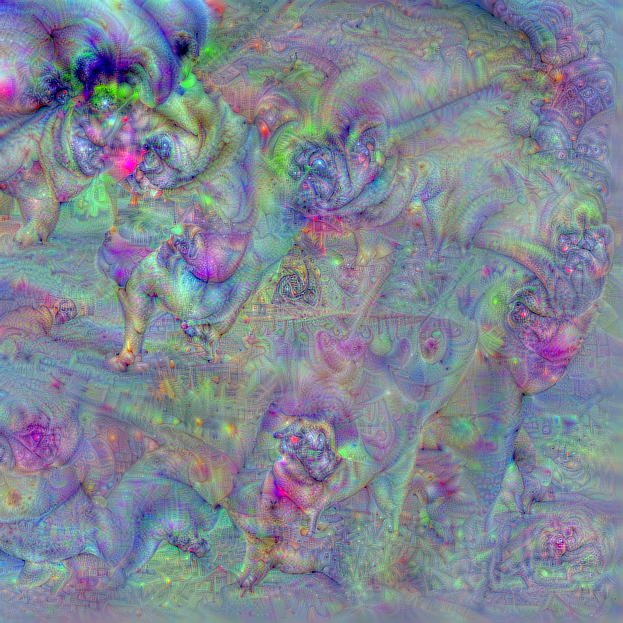
\includegraphics[width=.7\linewidth]{figuras/feat_vis/experiments/classes/cl254/random_image_ci254_lr8e-2_pl6.png}
        \caption{6 Layer Multiscaling, Blurring, \(learning\_rate = 0.08\)}
    \end{subfigure}

    \caption{Pug Class Feature Visualization for VGG16}
    \label{fig:class_pug}
\end{figure}

The generated images exhibit certain facial features of a Pug, including patterns that resemble its distinctive eyes and skin.

\subsubsection{Class 761 - Remote Control}

\begin{figure}
    \captionsetup{justification=centering}

    \begin{subfigure}[t]{0.31\textwidth}
        \captionsetup{justification=centering}
        \centering
        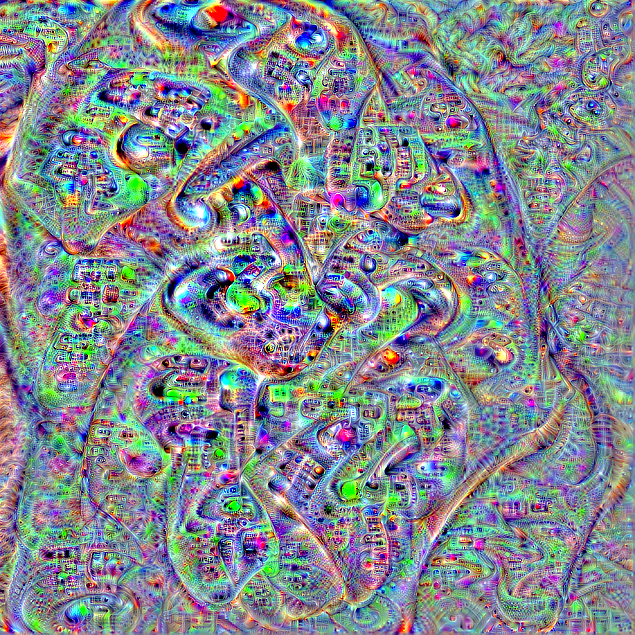
\includegraphics[width=.7\linewidth]{figuras/feat_vis/experiments/classes/cl761/random_image_ci761_lr1e-1_pl4_no-blur.png}
        \caption{4 Layer Multiscaling, No Blurring, \(learning\_rate = 0.1\)}
    \end{subfigure}
    \hfill
    \begin{subfigure}[t]{0.31\textwidth}
        \captionsetup{justification=centering}
        \centering
        \includegraphics[width=.7\linewidth]{figuras/feat_vis/experiments/classes/cl761/random_image_ci761_lr1e-1_pl6.png}
        \caption{6 Layer Multiscaling, Blurring, \(learning\_rate = 0.1\)}
    \end{subfigure}
    \hfill
    \begin{subfigure}[t]{0.31\textwidth}
        \captionsetup{justification=centering}
        \centering
        \includegraphics[width=.7\linewidth]{figuras/feat_vis/experiments/classes/cl761/random_image_ci761_lr4e-2_pl4.png}
        \caption{4 Layer Multiscaling, Blurring, \(learning\_rate = 0.04\)}
    \end{subfigure}

    \caption{Remote Controller Class Feature Visualization for VGG16}
    \label{fig:class_remote}
\end{figure}

The generated images do not strongly align with a human's typical perception of a remote controller. 
However, the convex shape with round patterns visible in image (c) might bear some resemblance to a remote controller.

\subsubsection{Class 771 - Safe}

\begin{figure}
    \captionsetup{justification=centering}

    \begin{subfigure}[t]{0.31\textwidth}
        \captionsetup{justification=centering}
        \centering
        \includegraphics[width=.7\linewidth]{figuras/feat_vis/experiments/classes/cl771/random_image_ci771_lr1e-2_pl6.png}
        \caption{6 Layer Multiscaling, Blurring, \(learning\_rate = 0.01\)}
    \end{subfigure}
    \hfill
    \begin{subfigure}[t]{0.31\textwidth}
        \captionsetup{justification=centering}
        \centering
        \includegraphics[width=.7\linewidth]{figuras/feat_vis/experiments/classes/cl771/random_image_ci771_lr4e-2_pl6.png}
        \caption{6 Layer Multiscaling, Blurring, \(learning\_rate = 0.04\)}
    \end{subfigure}
    \hfill
    \begin{subfigure}[t]{0.31\textwidth}
        \captionsetup{justification=centering}
        \centering
        \includegraphics[width=.7\linewidth]{figuras/feat_vis/experiments/classes/cl771/random_image_ci771_lr9e-2_pl4.png}
        \caption{4 Layer Multiscaling, Blurring, \(learning\_rate = 0.09\)}
    \end{subfigure}

    \caption{Safe Class Feature Visualization for VGG16}
    \label{fig:class_safe}
\end{figure}

Image (a) appears to have structures very similar to a safe, with a shape close to a square with a circle inside.
The generated images feature multiple straight lines and circular patterns, which are also found in the structures of safes.

\subsubsection{Class 783 - Screw}

\begin{figure}
    \captionsetup{justification=centering}

    \begin{subfigure}[t]{0.31\textwidth}
        \captionsetup{justification=centering}
        \centering
        \includegraphics[width=.7\linewidth]{figuras/feat_vis/experiments/classes/cl783/random_image_ci783_lr1e-1_pl4.png}
        \caption{4 Layer Multiscaling, Blurring, \(learning\_rate = 0.1\)}
    \end{subfigure}
    \hfill
    \begin{subfigure}[t]{0.31\textwidth}
        \captionsetup{justification=centering}
        \centering
        \includegraphics[width=.7\linewidth]{figuras/feat_vis/experiments/classes/cl783/random_image_ci783_lr4e-2_pl4_no-blur.png}
        \caption{4 Layer Multiscaling, No Blurring, \(learning\_rate = 0.04\)}
    \end{subfigure}
    \hfill
    \begin{subfigure}[t]{0.31\textwidth}
        \captionsetup{justification=centering}
        \centering
        \includegraphics[width=.7\linewidth]{figuras/feat_vis/experiments/classes/cl783/random_image_ci783_lr9e-2_pl6.png}
        \caption{6 Layer Multiscaling, Blurring, \(learning\_rate = 0.09\)}
    \end{subfigure}

    \caption{Screw Class Feature Visualization for VGG16}
    \label{fig:class_screw}
\end{figure}

Patterns very closely related to screws are present in the generated images, with screws in multiple positions and angles present in the generated content.

\newpage
\subsubsection{Class 817 - Sports Car}

\begin{figure}
    \captionsetup{justification=centering}

    \begin{subfigure}[t]{0.31\textwidth}
        \captionsetup{justification=centering}
        \centering
        \includegraphics[width=.7\linewidth]{figuras/feat_vis/experiments/classes/cl817/random_image_ci817_lr1e-1_pl6.png}
        \caption{6 Layer Multiscaling, Blurring, \(learning\_rate = 0.1\)}
    \end{subfigure}
    \hfill
    \begin{subfigure}[t]{0.31\textwidth}
        \captionsetup{justification=centering}
        \centering
        \includegraphics[width=.7\linewidth]{figuras/feat_vis/experiments/classes/cl817/random_image_ci817_lr8e-2_pl6.png}
        \caption{6 Layer Multiscaling, Blurring, \(learning\_rate = 0.08\)}
    \end{subfigure}
    \hfill
    \begin{subfigure}[t]{0.31\textwidth}
        \captionsetup{justification=centering}
        \centering
        \includegraphics[width=.7\linewidth]{figuras/feat_vis/experiments/classes/cl817/random_image_ci817_lr9e-2_pl6.png}
        \caption{6 Layer Multiscaling, Blurring, \(learning\_rate = 0.09\)}
    \end{subfigure}

    \caption{Sports Car Class Feature Visualization for VGG16}
    \label{fig:class_sports_car}
\end{figure}

Circles similar to wheels are present in the generated images, but not much resemblance is noticeable in the examples.

\subsubsection{Class 883 - Vase}

\begin{figure}
    \captionsetup{justification=centering}

    \begin{subfigure}[t]{0.31\textwidth}
        \captionsetup{justification=centering}
        \centering
        \includegraphics[width=.7\linewidth]{figuras/feat_vis/experiments/classes/cl883/random_image_ci883_lr1e-1_pl6.png}
        \caption{6 Layer Multiscaling, Blurring, \(learning\_rate = 0.1\)}
    \end{subfigure}
    \hfill
    \begin{subfigure}[t]{0.31\textwidth}
        \captionsetup{justification=centering}
        \centering
        \includegraphics[width=.7\linewidth]{figuras/feat_vis/experiments/classes/cl883/random_image_ci883_lr4e-2_pl6.png}
        \caption{6 Layer Multiscaling, Blurring, \(learning\_rate = 0.04\)}
    \end{subfigure}
    \hfill
    \begin{subfigure}[t]{0.31\textwidth}
        \captionsetup{justification=centering}
        \centering
        \includegraphics[width=.7\linewidth]{figuras/feat_vis/experiments/classes/cl883/random_image_ci883_lr8e-2_pl6.png}
        \caption{6 Layer Multiscaling, Blurring, \(learning\_rate = 0.08\)}
    \end{subfigure}

    \caption{Vase Class Feature Visualization for VGG16}
    \label{fig:class_vase}
\end{figure}

The sinuous shapes present in the images are very similar to a vase's structure.
It is possible to notice that the characteristic curve is present in multiple parts of the images.

\newpage
\subsubsection{Class 963 - Pizza}

\begin{figure}
    \captionsetup{justification=centering}

    \begin{subfigure}[t]{0.46\textwidth}
        \captionsetup{justification=centering}
        \centering
        \includegraphics[width=.7\linewidth]{figuras/feat_vis/experiments/classes/cl963/random_image_ci963_lr1e-1_pl4.png}
        \caption{4 Layer Multiscaling, Blurring, \(learning\_rate = 0.1\)}
    \end{subfigure}
    \hfill
    \begin{subfigure}[t]{0.46\textwidth}
        \captionsetup{justification=centering}
        \centering
        \includegraphics[width=.7\linewidth]{figuras/feat_vis/experiments/classes/cl963/random_image_ci963_lr1e-2_pl6.png}
        \caption{6 Layer Multiscaling, Blurring, \(learning\_rate = 0.01\)}
    \end{subfigure}
    \hfill
    \begin{subfigure}[t]{0.46\textwidth}
        \captionsetup{justification=centering}
        \centering
        \includegraphics[width=.7\linewidth]{figuras/feat_vis/experiments/classes/cl963/random_image_ci963_lr9e-2_pl4.png}
        \caption{4 Layer Multiscaling, Blurring, \(learning\_rate = 0.09\)}
    \end{subfigure}
    \hfill
    \begin{subfigure}[t]{0.46\textwidth}
        \captionsetup{justification=centering}
        \centering
        \includegraphics[width=.7\linewidth]{figuras/feat_vis/experiments/classes/cl963/random_image_ci963_lr9e-2_pl6.png}
        \caption{6 Layer Multiscaling, Blurring, \(learning\_rate = 0.09\)}
    \end{subfigure}

    \caption{Pizza Class Feature Visualization for VGG16}
    \label{fig:class_pizza}
\end{figure}

The images feature patterns reminiscent of melted cheese on a pizza, along with circular structures that evoke the classic pizza shape.
\subsection{Feature Visualization in Non-Random Initial Images}


Feature visualization techniques can also be applied to images with non-random initial states. 
By leveraging the methods discussed in this chapter, it becomes possible to create visuals that appear as if they were pulled directly from a \emph{dream}\footnotemark.
The following examples showcase images generated using this technique, illustrating its ability to produce dreamlike and surreal visuals.

\footnotetext{The idea of applying Feature Visualization to Non-Random Initial images became popular by a program called \emph{DeepDream}, created by Google}
\begin{figure}
    \captionsetup{justification=centering}

    \begin{subfigure}[t]{0.45\textwidth}
        \captionsetup{justification=centering}
        \centering
        \includegraphics[width=.7\linewidth]{figuras/feat_vis/experiments/non_random/christ-the-redeemer.jpg}
        \caption{Original Image}
    \end{subfigure}
    \hfill
    \begin{subfigure}[t]{0.45\textwidth}
        \captionsetup{justification=centering}
        \centering
        \includegraphics[width=.7\linewidth]{figuras/feat_vis/experiments/non_random/christ-the-redeemer_li24_lr8e-2_pl4.png}
        \caption{Feature Visualization of Image with Layer 11}
    \end{subfigure}

    \caption{Christ the Redeemer}
    \label{fig:christ_dream}
\end{figure}

\begin{figure}
    \captionsetup{justification=centering}

    \begin{subfigure}[t]{0.45\textwidth}
        \captionsetup{justification=centering}
        \centering
        \includegraphics[width=.7\linewidth]{figuras/feat_vis/experiments/non_random/ime-usp.jpg}
        \caption{Original Image}
    \end{subfigure}
    \hfill
    \begin{subfigure}[t]{0.45\textwidth}
        \captionsetup{justification=centering}
        \centering
        \includegraphics[width=.7\linewidth]{figuras/feat_vis/experiments/non_random/ime-usp_li24_lr4e-2_pl4_no-blur.png}
        \caption{Feature Visualization of Image with Layer 11}
    \end{subfigure}

    \caption{IME-USP}
    \label{fig:ime_dream}
\end{figure}

\begin{figure}
    \captionsetup{justification=centering}

    \begin{subfigure}[t]{0.45\textwidth}
        \captionsetup{justification=centering}
        \centering
        \includegraphics[width=.7\linewidth]{figuras/feat_vis/experiments/non_random/mona.jpg}
        \caption{Original Image}
    \end{subfigure}
    \hfill
    \begin{subfigure}[t]{0.45\textwidth}
        \captionsetup{justification=centering}
        \centering
        \includegraphics[width=.7\linewidth]{figuras/feat_vis/experiments/non_random/mona_li24_lr7e-2_pl4.png}
        \caption{Feature Visualization of Image with Layer 11}
    \end{subfigure}

    \caption{Mona Lisa}
    \label{fig:mona_dream}
\end{figure}

\begin{figure}
    \captionsetup{justification=centering}

    \begin{subfigure}[t]{0.45\textwidth}
        \captionsetup{justification=centering}
        \centering
        \includegraphics[width=.7\linewidth]{figuras/feat_vis/experiments/non_random/The-Great-Wave-off-Kanagawa.png}
        \caption{Original Image}
    \end{subfigure}
    \hfill
    \begin{subfigure}[t]{0.45\textwidth}
        \captionsetup{justification=centering}
        \centering
        \includegraphics[width=.7\linewidth]{figuras/feat_vis/experiments/non_random/The-Great-Wave-off-Kanagawa_li24_lr1e-2_pl4_no-blur.png}
        \caption{Feature Visualization of Image with Layer 11}
    \end{subfigure}

    \caption{The Great Wave off Kanagawa}
    \label{fig:wave_dream}
\end{figure}
